%%%%%%%%%%%%%%%%%%%%%%%%%%%%%%%%%%%%%%%%%
% Masters/Doctoral Thesis 
% LaTeX Template
% Version 2.5 (27/8/17)
%
% This template was downloaded from:
% http://www.LaTeXTemplates.com
%
% Version 2.x major modifications by:
% Vel (vel@latextemplates.com)
%
% This template is based on a template by:
% Steve Gunn (http://users.ecs.soton.ac.uk/srg/softwaretools/document/templates/)
% Sunil Patel (http://www.sunilpatel.co.uk/thesis-template/)
%
% Template license:
% CC BY-NC-SA 3.0 (http://creativecommons.org/licenses/by-nc-sa/3.0/)
%
%%%%%%%%%%%%%%%%%%%%%%%%%%%%%%%%%%%%%%%%%

%----------------------------------------------------------------------------------------
%	PACKAGES AND OTHER DOCUMENT CONFIGURATIONS
%----------------------------------------------------------------------------------------

\documentclass[
11pt, % The default document font size, options: 10pt, 11pt, 12pt
oneside, % Two side (alternating margins) for binding by default, uncomment to switch to one side
english, % ngerman for German
singlespacing, % Single line spacing, alternatives: onehalfspacing or doublespacing
%draft, % Uncomment to enable draft mode (no pictures, no links, overfull hboxes indicated)
% nolistspacing, % If the document is onehalfspacing or doublespacing, uncomment this to set spacing in lists to single
%liststotoc, % Uncomment to add the list of figures/tables/etc to the table of contents
%toctotoc, % Uncomment to add the main table of contents to the table of contents
%parskip, % Uncomment to add space between paragraphs
%nohyperref, % Uncomment to not load the hyperref package
headsepline, % Uncomment to get a line under the header
%chapterinoneline, % Uncomment to place the chapter title next to the number on one line
% consistentlayout, % Uncomment to change the layout of the declaration, abstract and acknowledgements pages to match the default layout
]{thesis} % The class file specifying the document structure

\usepackage[utf8]{inputenc} % Required for inputting international characters
\usepackage[T1]{fontenc} % Output font encoding for international characters
\usepackage{enumitem}
\usepackage{mathpazo} % Use the Palatino font by default
\usepackage[backend=bibtex,style=authoryear,natbib=true,maxbibnames=99]{biblatex} % Use the bibtex backend with the authoryear citation style (which resembles APA)
\usepackage[autostyle=true]{csquotes} % Required to generate language-dependent quotes in the bibliography
\usepackage{amsthm}
\usepackage{amsmath}
\usepackage{chngcntr}
\usepackage{threeparttable}
\usepackage{ragged2e}
\usepackage{algorithm} 
\usepackage{algpseudocode}
\usepackage{bm}
\usepackage{etoolbox}

\counterwithout{equation}{chapter}
\counterwithout{figure}{chapter}
\counterwithout{table}{chapter}
\theoremstyle{definition}
\newtheorem{definition}{Definition}
\theoremstyle{remark}
\newtheorem{remark}{Remark}[definition]
\addbibresource{../bibtex.bib} % The filename of the bibliography
\graphicspath{{../visuals/}}
\newcolumntype{L}[1]{>{\RaggedRight\hspace{0pt}}p{#1}}
\newcolumntype{R}[1]{>{\RaggedLeft\hspace{0pt}}p{#1}}
\renewcommand{\algorithmicrequire}{\textbf{Input(s):}}
\renewcommand{\algorithmicensure}{\textbf{Output(s):}}
\DeclareMathOperator*{\argmax}{arg\,max}
\algdef{SE}{Begin}{End}{\textbf{begin}}{\textbf{end}}
\algnewcommand\algorithmicforeach{\textbf{for each}}
\algdef{S}[FOR]{ForEach}[1]{\algorithmicforeach\ #1\ \algorithmicdo}

\makeatletter
\AfterEndEnvironment{algorithm}{\let\@algcomment\relax}
\AtEndEnvironment{algorithm}{\kern2pt\hrule\relax\vskip3pt\@algcomment}
\let\@algcomment\relax
\newcommand\algcomment[1]{\def\@algcomment{\footnotesize#1}}

\renewcommand\fs@ruled{\def\@fs@cfont{\bfseries}\let\@fs@capt\floatc@ruled
  \def\@fs@pre{\hrule height.8pt depth0pt \kern2pt}%
  \def\@fs@post{}%
  \def\@fs@mid{\kern2pt\hrule\kern2pt}%
  \let\@fs@iftopcapt\iftrue}
\makeatother

%----------------------------------------------------------------------------------------
%	MARGIN SETTINGS
%----------------------------------------------------------------------------------------

\geometry{
	paper=a4paper, % Change to letterpaper for US letter
	inner=2.5cm, % Inner margin
	outer=3.8cm, % Outer margin
	bindingoffset=.5cm, % Binding offset
	top=1.5cm, % Top margin
	bottom=1.5cm, % Bottom margin
	%showframe, % Uncomment to show how the type block is set on the page
}

%----------------------------------------------------------------------------------------
%	THESIS INFORMATION
%----------------------------------------------------------------------------------------

\thesistitle{SoPa++: Leveraging explainability from hybridized RNN, CNN and weighted finite-state neural architectures} % Your thesis title, this is used in the title and abstract, print it elsewhere with \ttitle
\supervisor{Dr. Sharid \textsc{Loáiciga} \\ University of Potsdam} % Your supervisor's name, this is used in the title page, print it elsewhere with \supname
\examiner{Mathias \textsc{Müller} \\ University of Zurich} % Your examiner's name, this is not currently used anywhere in the template, print it elsewhere with \examname
\degree{Cognitive Systems: Language, \\ Learning, and Reasoning (M.Sc.)} % Your degree name, this is used in the title page and abstract, print it elsewhere with \degreename
\author{Atreya \textsc{Shankar} \\ 799227} % Your name, this is used in the title page and abstract, print it elsewhere with \authorname
\addresses{} % Your address, this is not currently used anywhere in the template, print it elsewhere with \addressname

\subject{Computational Linguistics} % Your subject area, this is not currently used anywhere in the template, print it elsewhere with \subjectname
\keywords{} % Keywords for your thesis, this is not currently used anywhere in the template, print it elsewhere with \keywordnames
\university{\href{https://www.uni-potsdam.de/en/university-of-potsdam}{University of Potsdam}} % Your university's name and URL, this is used in the title page and abstract, print it elsewhere with \univname
\department{\href{https://www.uni-potsdam.de/en/ling/index}{Department of Linguistics}} % Your department's name and URL, this is used in the title page and abstract, print it elsewhere with \deptname
\group{\href{http://clp.ling.uni-potsdam.de/}{Foundations of Computational Linguistics Research Group
}} % Your research group's name and URL, this is used in the title page, print it elsewhere with \groupname

\AtBeginDocument{
\hypersetup{pdftitle=\ttitle} % Set the PDF's title to your title
\hypersetup{pdfauthor=\authorname} % Set the PDF's author to your name
\hypersetup{pdfkeywords=\keywordnames} % Set the PDF's keywords to your keywords
}

\begin{document}

\frontmatter % Use roman page numbering style (i, ii, iii, iv...) for the pre-content pages

\pagestyle{plain} % Default to the plain heading style until the thesis style is called for the body content

%----------------------------------------------------------------------------------------
%	TITLE PAGE
%----------------------------------------------------------------------------------------

\begin{titlepage}
\begin{center}

\vspace*{.06\textheight}
{\scshape\LARGE \univname\par}\vspace{1.5cm} % University name
\textsc{\Large Master's Thesis}\\[0.5cm] % Thesis type

\HRule \\[0.4cm] % Horizontal line
{\huge \bfseries \ttitle\par}\vspace{0.4cm} % Thesis title
\HRule \\[1.5cm] % Horizontal line
 
\begin{minipage}[t]{0.4\textwidth}
\begin{flushleft} \large
\emph{Author:}\\
\href{https://www.linkedin.com/in/atreya-shankar-644352113}{\authorname} % Author name - remove the \href bracket to remove the link
\end{flushleft}
\end{minipage}
\begin{minipage}[t]{0.4\textwidth}
\begin{flushright} \large
\emph{1st Supervisor:} \\
\href{https://sites.google.com/site/loaicigasharid/portada}{\supname} \\[10pt] % Supervisor name - remove the \href bracket to remove the link
\emph{2nd Supervisor:} \\
\href{https://www.uzh.ch/cmsssl/cl/de/people/team/compling/mmueller.html}{\examname} % Supervisor name - remove the \href bracket to remove the link  
\end{flushright}
\end{minipage}\\[3cm]
 
\vfill

\large \textit{A thesis submitted in fulfillment of the requirements\\ for the degree of \degreename}\\[0.3cm] % University requirement text
\textit{in the}\\[0.4cm]
\groupname\\\deptname\\[2cm] % Research group name and department name
 
\vfill

{\large \today}\\[4cm] % Date
% \includegraphics[width=5cm]{images/UP.jpg} % University/department logo - uncomment to place it
 
\vfill
\end{center}
\end{titlepage}

%----------------------------------------------------------------------------------------
%	LIST OF CONTENTS/FIGURES/TABLES PAGES
%----------------------------------------------------------------------------------------

\tableofcontents % Prints the main table of contents

%----------------------------------------------------------------------------------------
%	THESIS CONTENT - CHAPTERS
%----------------------------------------------------------------------------------------

\mainmatter % Begin numeric (1,2,3...) page numbering

\pagestyle{thesis} % Return the page headers back to the "thesis" style

% Include the chapters of the thesis as separate files from the Chapters folder
% Uncomment the lines as you write the chapters

\chapter{Introduction}

\label{chapter:introduction}

In this chapter, we introduce this thesis by presenting its motivation,
describing our research questions and providing an overview of the thesis
structure.

\section{Motivation and objective}

There is a recent trend of increasingly complex deep learning models achieving
state-of-the-art performance on \ac{ml} and \ac{nlp} tasks, as shown in Figure
\ref{fig:nlp_progress}. To address emerging concerns such as security risks and
inductive biases, several studies argue for focused research into \ac{xai}
\citep{doran2017does,townsend2019extracting,danilevsky2020survey,arrieta2020explainable}.
Of these studies, \citet{arrieta2020explainable} provide an extensive overview
of \ac{xai} and related concepts based on a thorough literature review of
$\sim$400 \ac{xai} research contributions published to date. In particular,
\citet{arrieta2020explainable} explore and classify a variety of \ac{ml} models
into transparent and black-box categories depending on their degrees of
transparency. Furthermore, they explore taxonomies of post-hoc explainability
techniques aimed at effectively explaining black-box models. Notable
explainability techniques used in recent research include local explanations,
feature relevance and explanations by simplification.

Through our own survey of recent literature on explainability techniques in
\ac{nlp}, we came across several interesting studies employing the three
aforementioned post-hoc explainability techniques to better explain deep neural networks
\citep{schwartz2018sopa,peng2018rational,suresh-etal-2019-distilling,wang2019state,jiang2020cold}.
Of these studies, we draw inspiration from \citet{schwartz2018sopa} who
developed the novel hybridized \ac{rnn}, \ac{cnn} and weighted finite-state
\ac{sopa} model architecture with a special focus in model explainability. While
the \ac{sopa} model functions well, we find its explainability techniques to be
localized and indirect despite its neural architecture being suited for the
globalized and direct explanations by simplification explainability technique.
The main objective of this thesis is to address these limitations and to propose
a modified model, \textbf{\ac{spp}}, which could allow for effective explanations
by simplification. To facilitate this objective, we study both the performance and
explanations by simplification of the modified \ac{spp} model on the recently
released \ac{fmtod} data set from \citet{schuster-etal-2019-cross-lingual};
focusing on the English-language intent classification task.

\begin{figure}[t!]
  \centering
  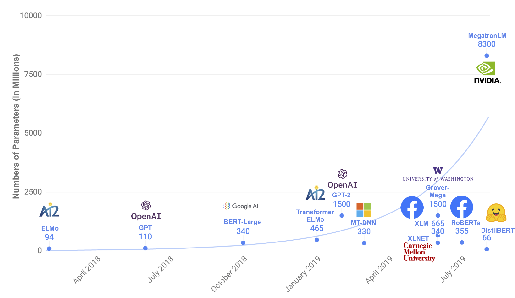
\includegraphics[width=13cm]{pdfs/borrowed/nlp_sota_model_size_progress.pdf}
  \caption{Parameter counts of recently released pre-trained language models
    which showed competitive or state-of-the-art performance when fine-tuned
    over a range of NLP tasks; figure taken from \citet{sanh2019distilbert}}
  \label{fig:nlp_progress}
\end{figure}

\section{Research questions}

\label{section:rq}

To guide us in addressing our objective, we aim to answer the following three
research questions:

\begin{enumerate}
  \item Does \ac{spp} provide competitive\footnote{We define
    competitive performance as the scenario where a mean performance metric on a
    certain task falls within the range obtained from other recent studies on
    the same task} performance on the \ac{fmtod} English language intent classification task?
  \item To what extent does \ac{spp} contribute to effective explanations by
  simplification on the \ac{fmtod} English language intent classification task?
  \item What interesting and relevant explanations can \ac{spp} provide on the
  \ac{fmtod} English language intent classification task?
\end{enumerate}

\section{Thesis structure}

We now summarize the contents and structure of this thesis.

\begin{description}[align=left]
  \item [Chapter \ref{chapter:introduction}:] Introduce this thesis, its
  contents and our research questions.
  \item [Chapter \ref{chapter:background}:] Describe the background concepts
  utilized in this thesis.
  \item [Chapter \ref{chapter:methodologies}:] Describe the \ac{fmtod} data set and
  methodologies pursued in this thesis.
  \item [Chapter \ref{chapter:results}:] Describe the results obtained from our
  methodologies.
  \item [Chapter \ref{chapter:discussion}:] Interpret the results and discuss their
  implications.
  \item [Chapter \ref{chapter:conclusions}:] Summarize the findings
  of this thesis.
  \item [Chapter \ref{chapter:further_work}:] Describe future work to expand on
  our research questions.
\end{description}

% LocalWords:  explainability pre NLP

%%% Local Variables: 
%%% mode: latex
%%% TeX-master: "main"
%%% End:
\chapter{Background concepts}

\label{chapter:background}

In this chapter, we describe the various background concepts necessary to
support the methodologies pursued in this thesis. These background concepts
range from conceptualizations and definitions in \ac{xai}, variants of
finite-state automata, straight-through estimators and finally the \ac{sopa}
model framework.

\section{Explainable artificial intelligence}

\label{section:xai}

In this section, we lay out background concepts for \ac{xai} which have been
largely adapted from \citet{arrieta2020explainable}. The study is especially
helpful for us since it summarizes the findings of $\sim$400 \ac{xai}
contributions and presents these findings in the form of well-defined concepts
and taxonomies. In addition, this study discusses many possible future
directions of \ac{xai} research.

\subsection{Transparency}

A key contribution of \citet{arrieta2020explainable} to the field of
\ac{xai} is the introduction of the concept of transparency, as well as the
classification of various \ac{ml} models into transparent and
black-box categories. In this section, we provide an adapted definition of
transparency and list examples of transparent and black-box \ac{ml} models.

\begin{definition}[Transparency; \citealt{arrieta2020explainable}; Page 4,
  Section 2.1]
  A model is considered to be transparent if it is understandable on its own
  without any external techniques to assist its understandability. Since a model
  can provide different degrees of understandability, transparent models are
  split into three possibly overlapping categories; specifically
  simulatable models, decomposable models and algorithmically transparent
  models.
\end{definition}

\begin{remark}
  \textit{Simulatability} refers to the ability of a model's inner-mechanisms
  being simulated strictly by a human. Therefore, model simplicity plays a major
  role in this class \citep[Page 6, Section 2.5.1]{arrieta2020explainable}.
\end{remark}

\begin{remark}
  \textit{Decomposability} refers to the ability to clearly understand the
  individual parts of a model; such as its inputs, parameters and basic
  computational mechanisms \citep[Page 7, Section 2.5.1]{arrieta2020explainable}.
\end{remark}

\begin{remark}
  \textit{Algorithmic transparency} refers to the ability of a human to
  understand the algorithmic processes used in the model to produce any given
  output from any given input \citep[Page 7, Section 2.5.1]{arrieta2020explainable}.
\end{remark}

\begin{remark}
  A model is considered transparent if it falls into one or more of the
  aforementioned transparency categories. If a model cannot satisfy any of the
  requirements of being transparent, then it is classified as a
  \textit{black-box} model \citep[Page 7, Section 3]{arrieta2020explainable}.
\end{remark}

\begin{remark}
  \label{rmk:equivalence}
  As recommended by \citet[Page 3, Section 2.1]{arrieta2020explainable}, we use
  the terms \textit{transparency} and \textit{interpretability} to refer to the same feature.
  Therefore, we use these terms equivalently and interchangeably.
\end{remark}

Examples of well-known transparent \ac{ml} models are linear/logistic
regressors, decision trees and rules-based learners. Similarly, common examples
of black-box \ac{ml} models are tree ensembles and deep neural networks.
\citet[Page 7, Section 3]{arrieta2020explainable} provide extensive
justifications using the aforementioned three criteria in conducting model
classifications into the transparent and black-box categories. We would direct
the reader to their study for a full analysis and justification of these
classifications.

\subsection{Explainability and XAI}

Another key contribution of \citet{arrieta2020explainable} is a unified
conceptualization of explainability and \ac{xai}. Drawing inspiration from their
study, we provide adapted definitions of explainability and \ac{xai}, as well as
comment on interesting aspects related to \ac{xai}.

\begin{definition}[Explainability; \citealt{arrieta2020explainable}; Page 4,
  Section 2.1]
  Explainability refers to the interface between humans and a model, such that
  this interface is both an accurate proxy of the model and comprehensible to
  humans.
\end{definition}

\begin{definition}[Explainable Artificial Intelligence;
  \citealt{arrieta2020explainable}; Page 4, Section 2.2]
  An explainable artificial intelligence is one that produces details to make
  its functioning understandable to a given target audience.
\end{definition}

\citet[Page 2, Section 1]{arrieta2020explainable} observe that black-box \ac{ml}
models are increasingly being employed to make important predictions in critical
contexts, citing high-risk areas such as precision medicine and autonomous
vehicles. Of particular relevance to the field of \ac{nlp}, the study notes a
myriad of issues related to inductive biases within training data sets and the
ethical issues involved in using black-box models trained on such data sets. As
a result, they describe an increased demand for explainability in black-box
\ac{ml} models from the various stakeholders in Artificial Intelligence. In
addition, \citet[Page 4, Section 2.2]{arrieta2020explainable} emphasize the
presence of a target audience for \ac{xai}; implying that different \ac{xai}
techniques should be employed for different target audiences. In their study,
they provide examples of target audiences such as domain experts, end-users and
managers as shown in Figure \ref{fig:xai_target_audience}.

\begin{figure}[t]
  \centering 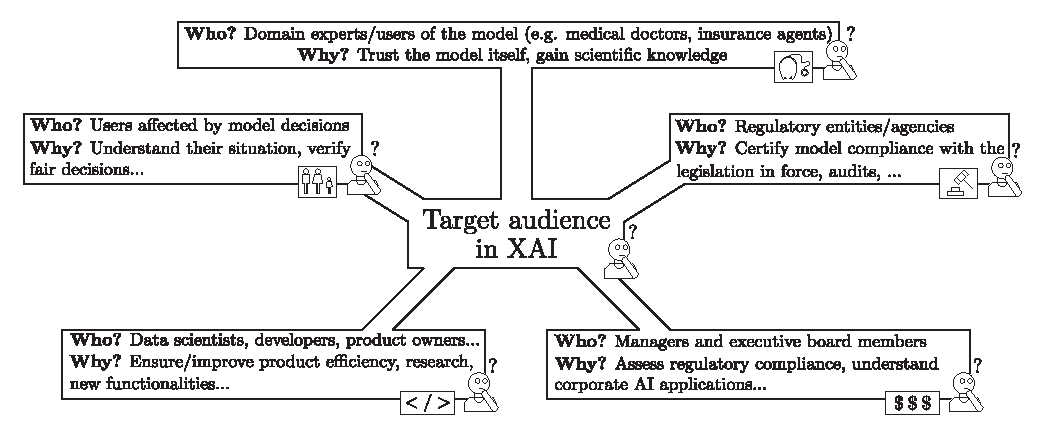
\includegraphics[trim={0.1cm 0.1cm 0.1cm
    0.1cm},clip,width=14cm]{pdfs/borrowed/xai_target_audience.pdf}
  \caption{Examples of various target audiences in XAI; figure taken from
    \citet{arrieta2020explainable}}
  \label{fig:xai_target_audience}
\end{figure}

\subsection{Terminology clarification}

\label{section:xai_terminology}

\citet{arrieta2020explainable} observe that many studies in XAI tend to misuse the
terms interpretability and explainability by using them interchangeably. To
address this, they provide clear conceptual differences between the terms. For
example, \citet[Page 3, Section 2.1]{arrieta2020explainable} state that
\textit{``interpretability refers to a passive characteristic of a model
  referring to the level at which a given model makes sense for a human
  observer.''} In contrast, \citet[Page 3, Section 2.1]{arrieta2020explainable}
state that \textit{``explainability can be viewed as an active characteristic of
  a model, denoting any action or procedure taken by a model with the intent of
  clarifying or detailing its internal functions.''}

In summary, we gather that interpretability (or transparency as per Remark
\ref{rmk:equivalence}) refers to an inherent or passive feature of a model. On
the other hand, explainability refers to an active characteristic undertaken by
the model and its developers to explain the model's inner mechanisms. In
addition, explainability entails the presence of a target audience; which may
not necessarily be the case for interpretability or transparency.

\subsection{Post-hoc explainability techniques}

\label{section:xai_techniques}

Based on the aforementioned classification of \ac{ml} models into transparent and
black-box models, \citet{arrieta2020explainable} expound on explainability
techniques for each of these model types. Due to their transparent nature, the
study states that transparent \ac{ml} models are usually explainable in themselves to
most target audiences and therefore usually do not require any external
technique to extract explanations. The study does however highlight some target
audiences, such as non-expert users, who may require external explainability
techniques such as model output visualizations in order to explain the inner
workings of transparent \ac{ml} models.

For the case of black-box models, \citet{arrieta2020explainable} argue that
separate or external techniques must be utilized in order to reasonably explain
these models. Such explainability techniques are referred to in the study as
post-hoc explainability techniques; which is derived from the idea that
explanations for such models are usually extracted post-modeling. Notable
post-hoc explainability techniques used in recent research include local
explanations, feature relevance and explanations by simplification; for which we
provide adapted definitions below.

\begin{definition}[Local explanations; \citealt{arrieta2020explainable}; Page 11,
  Section 4.1]
  Local explanations operate by segmenting a model's solution space into
  subspaces and provide explanations for the less complex model subspaces.
\end{definition}

\begin{remark}
  Local explanations are commonly used in \ac{xai} research and function by using
  differentiating properties on model solution space subsets \citep[Page 7,
  Section 2.5.2]{arrieta2020explainable}.
\end{remark}

\begin{remark}
  Two well-known examples of local explainability techniques are Local
  Interpretable Model-Agnostic Explanations \citep{lime} and G-REX
  \citep{konig2008g}.
\end{remark}

\begin{definition}[Feature relevance; \citealt{arrieta2020explainable}; Page 11,
  Section 4.1]
  Feature relevance explanation methods operate by computing an importance score
  for the model's input features over the model's outputs. These
  scores typically quantify how sensitive the model's output is to perturbations
  in the model's inputs or internal features.
\end{definition}

\begin{remark}
  \label{rmk:feature_relevance_indirect}
  Feature relevance methods can be considered as indirect methods of explaining
  a model \citep[Page 7, Section 2.5.2]{arrieta2020explainable}.
\end{remark}

\begin{remark}
  Well-known feature relevance explainability techniques include the Shapley
  Additive Explanations \citep{lundberg2017unified} and the occlusion
  sensitivity method \citep{zeiler2014visualizing}.
\end{remark}

\begin{definition}[Explanations by simplification;
  \citealt{arrieta2020explainable}; Page 11, Section 4.1]
  \label{def:explain_simplify}
  Explanations by simplification refer to techniques where a simplified proxy
  model is built to approximate and explain a more complex model. The simplified
  proxy model usually has to fulfill the joint criteria of reducing its
  complexity compared to its antecedent model while maximizing its resemblance
  to its antecedent and keeping a similar performance score.
\end{definition}

\begin{remark}
  In this thesis, we refer to the original black-box model as an
  \textit{antecedent} model and the simplified model as the \textit{proxy}
  model. Furthermore, we qualify that all proxy models must be designed to
  globally approximate their respective antecedent models.
\end{remark}

\begin{remark}
  \citet{bastani2017interpretability} and \citet{tan2018distill} are examples of
  studies that extract and distill simpler proxy models from complex antecedent
  models.
\end{remark}

Through our own survey of recent literature on explainability techniques used in
\ac{nlp}, we came across several interesting studies employing the local
explanations, feature relevance and explanations by simplification
explainability techniques to better explain black-box models; particularly deep
neural networks
\citep{schwartz2018sopa,peng2018rational,suresh-etal-2019-distilling,wang2019state,jiang2020cold}.
We expound more on these in Sections \ref{section:fa} and \ref{section:sopa}
respectively.

\begin{figure}[t]
  \centering
  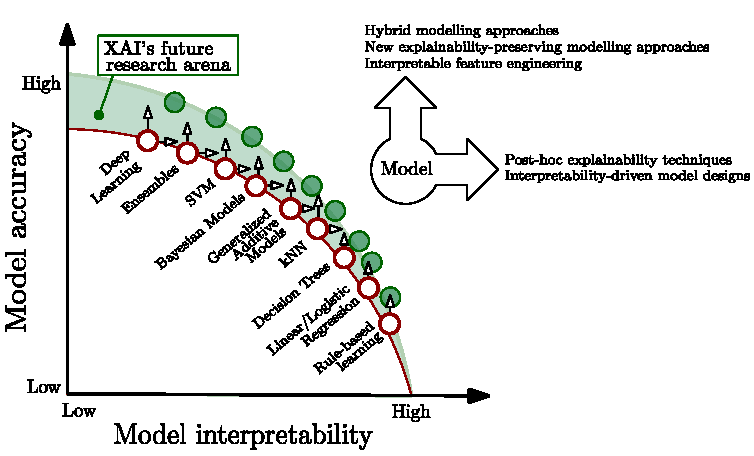
\includegraphics[width=14cm]{pdfs/borrowed/performance_transparency_tradeoff.pdf}
  \caption{Qualitative visualization of the performance-interpretability tradeoff;
    figure taken from \citet{arrieta2020explainable}}
  \label{fig:performance_interpretability_tradeoff}
\end{figure}

\subsection{Performance-interpretability tradeoff}

\label{section:performance_interpretability_tradeoff}

An interesting and insightful contribution of \citet{arrieta2020explainable} is
their conceptualization of the performance-interpretability tradeoff; which in
its essence states that the interpretability or transparency of models is
negatively correlated with performance on \ac{ml} tasks. \citet[Page 18, Section
5.1]{arrieta2020explainable} introduce the performance-interpretability tradeoff
with the caveat that \textit{``the matter of interpretability versus performance
  is one that repeats itself through time, but as any other big statement, has
  its surroundings filled with myths and misconceptions.''} To address some of
the aforementioned myths and misconceptions, \citet{arrieta2020explainable}
first disprove the generic statement that black-box models are
\textit{always} more performant by pointing to case studies which show that
transparent models can perform on-par or better than black-box models when the
function to be modeled is simple, data is well-structured and input
features are available with high quality.

With these exceptions clarified, \citet{arrieta2020explainable} then provide cases
which show that black-box models perform better than transparent models; which
ultimately gives rise to the performance-interpretability tradeoff as
reflected in Figure \ref{fig:performance_interpretability_tradeoff}. According to
them, this is usually the case when the function to be modeled is sufficiently
complex and where the input data has high diversity or variance; and possibly
contains significant noise.

\subsection{Explainability metrics}

\label{section:xai_metrics}

Towards the end of their study, \citet{arrieta2020explainable} note two major
limitations of the current state of \ac{xai} research. Firstly, \citet[Page 19,
Section 5.2]{arrieta2020explainable} observe the lack of a unified
conceptualization of explainability and transparency between various studies. To
address this, they acknowledge that their study could provide a good unified
starting point for other \ac{xai} studies to branch out from. Secondly,
\citet[Page 20, Section 5.3]{arrieta2020explainable} note the lack of a unified
metric that denotes how explainable any given model is. They explain why
developing such a metric has been a difficult process for many \ac{xai} studies;
particularly because such a metric would entail incorporating psychological,
sociological and cognitive elements to accommodate the goodness of fit of an
explainability technique to a certain target audience. Furthermore,
incorporating such elements might involve significant amounts of subjectivity in
the desired metric.

To reduce some of the aforementioned subjectivity involved, \citet[Page 3,
Section 1.2]{MILLER20191} and \citet[Page 20, Section
5.3]{arrieta2020explainable} provide three guidelines of what could constitute a
good explanation based on human psychology, sociology and cognitive sciences:

\begin{enumerate}
  \item Firstly, they observe that explanations are better when
  \textit{constrictive}; meaning an explanation is good if it not only explains
  why a model made decision X, but also why it made decision X over decision Y.

  \item Next, they suggest that good explanations should be able to communicate
  \textit{causal} links over probabilities; which could be a challenge for black-box
  models which generally compute aggregate probabilities without necessarily
  considering causal links.

  \item Finally, they recommend that explanations are better when
  \textit{selective}; meaning that a good explanation should be able to
  selectively provide the most important causal links instead of all possible
  causal links as these might be irrelevant or confusing to the target audience.
\end{enumerate}

\section{Straight-through estimator}

\label{section:ste}

Quantized neural networks refer to neural networks that contain
layers which transmit piecewise discrete signals and have been an object of
active research in regards to low-precision and low-resource computing. One of
the main challenges in training such quantized neural networks is
that their gradients tend to vanish almost everywhere because the derivatives of
such piecewise discrete activation functions typically default to zero
\citep{bengio2013estimating,courbariaux2016binarized,yin2019understanding}.

One significant workaround for this issue was proposed by
\citet{bengio2013estimating} through the introduction of the \ac{ste}. In the
vanilla version of the \ac{ste}, the \ac{ste} neuron emits a signal of 1 when its input is
strictly positive, and emits a zero signal in all other cases (Equation
\ref{eq:ste_forward}). The \ac{ste} then uses a simple identity function to estimate
the gradient during the backward pass (Equation \ref{eq:ste_backward}). The
vanilla \ac{ste} is visualized in Figure \ref{fig:ste}.

\begin{equation}
  \label{eq:ste_forward}
  \text{STE}(x)=
  \begin{cases}
    1 & x \in (0, +\infty) \\
    0 & x \in (-\infty, 0]
  \end{cases}
\end{equation}

\begin{equation}
  \label{eq:ste_backward}
  \text{STE}'(x)= x
\end{equation}

\begin{figure}[t]
  \centering
  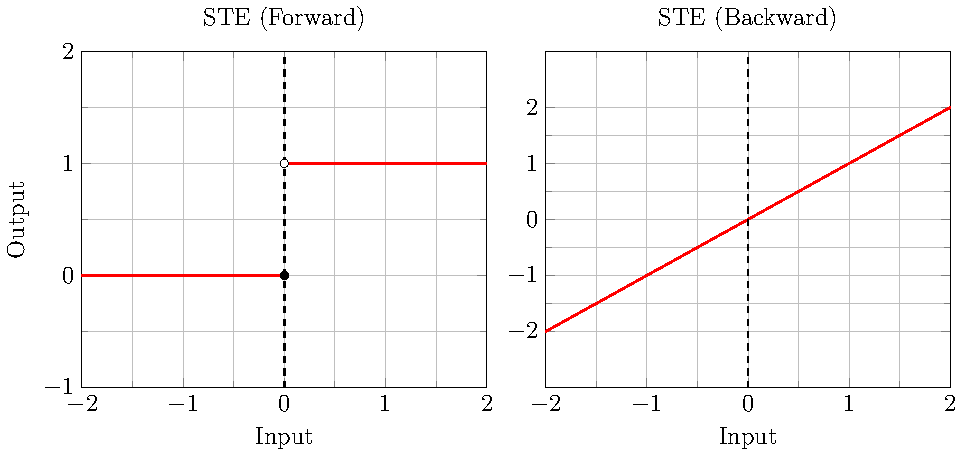
\includegraphics[width=14cm]{pdfs/generated/ste_theoretical/main.pdf}
  \caption{Vanilla STE's forward and backward passes}
  \label{fig:ste}
\end{figure}

Aside from the vanilla \ac{ste}, several other flavors of \ac{ste}s have been proposed by
studies such as \citet{courbariaux2016binarized} and
\citet{yin2019understanding}. In general, these studies have shown that
quantized neural networks perform competitively with their
non-quantized counterparts; while providing performance-related benefits related
to lower precision computing as well as enabling further research into threshold
driven neural activation functions.

\section{Finite-state automata}

\label{section:fa}

As mentioned in Section \ref{section:xai_techniques}, our survey of
explainability in \ac{nlp} yielded several studies employing post-hoc
explainability techniques on deep neural networks. One common factor among
several of these studies was the simplification of black-box models to
\ac{fas}. As this will eventually become a key focus of this
thesis, we define key concepts related to the \ac{fas}; as well as extensions to \ac{fas}.

\subsection{Finite-state automaton}

Finite-state automata is a collective term for two sub-categories of models;
namely deterministic and nondeterministic finite-state automata. Here we provide
definitions and descriptions for these mutually exclusive model categories.

\begin{definition}[Deterministic finite-state automaton;
  \citealt{sipser1996introduction}]
  \label{def:fa}
  A deterministic finite-state automaton is a 5-tuple $\mathcal{M} = \langle
  \Sigma, \mathcal{Q}, \delta, q_0, F \rangle$, with:
  \begin{itemize}
    \itemsep0em
    \item[--] a finite input alphabet $\Sigma$;
    \item[--] a finite state set $\mathcal{Q}$;
    \item[--] a transition function $\delta: \mathcal{Q} \times \Sigma
    \rightarrow \mathcal{Q}$;
    \item[--] an initial state $q_0 \in \mathcal{Q}$;
    \item[--] and a set of final or accepting states $F \subseteq Q$.
  \end{itemize}
\end{definition}

\begin{definition}[Nondeterministic finite-state automaton;
  \citealt{sipser1996introduction}]
  \label{def:nfa}
  A nondeterministic finite-state automaton is a 5-tuple $\mathcal{M} = \langle
  \Sigma, \mathcal{Q}, \delta, q_0, F \rangle$, with:
  \begin{itemize}
    \itemsep0em
    \item[--] a finite input alphabet $\Sigma$;
    \item[--] a finite state set $\mathcal{Q}$;
    \item[--] a transition function $\delta: \mathcal{Q} \times \{\Sigma \cup
    \{\epsilon\}\} \rightarrow \mathcal{P}(\mathcal{Q})$;
    \item[--] an initial state $q_0 \in \mathcal{Q}$;
    \item[--] and a set of final or accepting states $F \subseteq Q$.
  \end{itemize}

  \begin{remark}
    $\epsilon \notin \Sigma$ refers to an empty-string transition
    and results in a change of state without consuming any input
    token. These transitions are unique to nondeterministic finite-state automata.
  \end{remark}

  \begin{remark}
    Self-loop transitions refer to special transitions which consume an input token
    while staying at the same state. These are allowed in both deterministic and
    nondeterministic finite-state automata.
  \end{remark}
  
  \begin{remark}
    $\mathcal{P}(\mathcal{Q})$ refers to the power set of $\mathcal{Q}$, or
    otherwise the collection of all subsets of $\mathcal{Q}$.
  \end{remark}
\end{definition}

\begin{definition}[Linear-chain finite-state automaton;
  \citealt{schwartz2018sopa}]
  \label{def:lfa}
  Any finite-state automaton is considered linear-chain if there exists only one
  set of consecutive transition states leading from the start to the accepting
  state. Linear-chain finite-state automata furthermore possess only one start
  and accepting state and only allow transitions to the same or next state which is
  closer to the accepting state.

  \begin{remark}
    \label{rmk:strict_linear_chain}
    A linear-chain finite-state automaton can be considered as \textit{strict}
    if it does not permit self-loop transitions and therefore only permits
    transitions to adjacent states which are strictly closer to the
    accepting state. An example of a strict linear-chain \ac{nfa} can be seen in
    Figure \ref{fig:regex_fa}.
  \end{remark}

  \begin{remark}
    The presence of the linear-chain terminology is effectively absent in
    theoretical computer science literature but is prevalent in practical
    research related to Hidden Markov Models and Conditional Random
    Fields such as in \citet{tsuruoka2009fast}. As a result, we are only
    able to provide a text-based definition here.
  \end{remark}
  
\end{definition}

A string $\bm{x}$ is said to be \textit{accepted} by any \ac{fa} $\mathcal{M}$
if the current state after consuming string $\bm{x}$ is the accepting state.
Similarly, a string $\bm{x}$ is said to be \textit{rejected} by any \ac{fa}
$\mathcal{M}$ if the string $\bm{x}$ cannot be consumed or the current state
after consuming $\bm{x}$ is a non-accepting state. The key difference between
deterministic \ac{fas} and nondeterministic \ac{fas} is present in their
transition functions; specifically that the former guarantees that each state
allows for a unique transition to another state given a non-empty input token.
Contrastingly, \ac{nfas} allow for arbitrary transitions without necessarily
consuming an input token.

\begin{figure}[t]
  \centering
  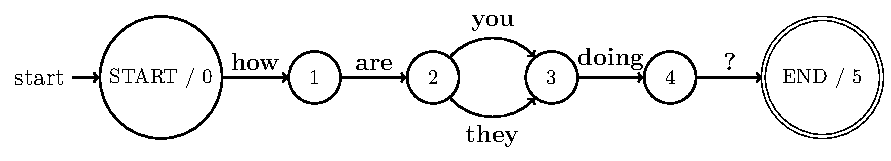
\includegraphics[width=14cm]{pdfs/generated/re_nfa_linear_chain/main.pdf}
  \caption{Regular expression \texttt{``how are (you|they) doing ?''} converted
    into a strict linear-chain NFA; double circles on state 5 indicate an
    accepting state}
  \label{fig:regex_fa}
\end{figure}

\subsection{Regular expressions}

Regular expressions and \ac{fas} have been shown to be equivalent in their
expressive power in that they both recognize regular languages
\citep{sipser1996introduction}. Historically, several algorithms have been
studied and optimized for converting \ac{fas} to regular expressions and vice-versa
\citep{mcnaughton1960regular,thompson1968programming}. Figure \ref{fig:regex_fa}
shows a simple example of converting the regular expression \texttt{``how are
  (you|they) doing ?''} into a strict linear-chain \ac{nfa}. The aforementioned
regular expression is written using the Perl-compatible regular expression
syntax with the \texttt{``|''} character indicating alternative possibilities.

\subsection{Weighted finite-state automaton}

\ac{wfas} are extensions of finite-state automata
which allow for the assignment of numerical weights to transitions given a
semiring to govern the algebra of the transitions. Compared to
the aforementioned \ac{fas} that only accept or reject strings, \ac{wfas} numerically
score strings which has made them useful for several applications in \ac{nlp} such as
tokenization and part-of-speech tagging \citep{maletti2017survey}. Here, we provide
extensive definitions of a semiring, \ac{wfa}, path score and string score.

\begin{definition}[Semiring; \citealt{kuich1986linear}]
  \label{def:semiring}
  A semiring is a set $\mathbb{K}$ along with two binary associative operations
  $\oplus$ (addition) and $\otimes$ (multiplication) and two identity elements:
  $\bar{0}$ for addition and $\bar{1}$ for multiplication. Semirings require
  that addition is commutative, multiplication distributes over addition, and
  that multiplication by $\bar{0}$ annihilates, i.e., $\bar{0} \otimes a = a
  \otimes \bar{0} = \bar{0}$.

\begin{remark}
  Semirings follow the following generic notation: $\langle \mathbb{K}, \oplus,
  \otimes, \bar{0}, \bar{1} \rangle$.
\end{remark}

\begin{remark}
  A simple and common semiring is the real or sum-product semiring: $\langle
  \mathbb{R}, +, \times, 0, 1 \rangle$. Two important semirings for this thesis
  are shown below.
\end{remark}

\begin{remark}
  \textbf{Max-sum} semiring: $\langle \mathbb{R} \cup \{-\infty\}, \text{max},
  +, -\infty, 0 \rangle$
\end{remark}

\begin{remark}
  \textbf{Max-product} semiring: $\langle \mathbb{R}_{>0} \cup \{-\infty\},
  \text{max}, \times, -\infty, 1 \rangle$
\end{remark}

\end{definition}

\begin{definition}[Weighted finite-state automaton; \citealt{peng2018rational}]
  \label{def:wfa}
  A weighted finite-state automaton over a semiring $\mathbb{K}$ is a 5-tuple
  $\mathcal{A} = \langle \Sigma, \mathcal{Q}, \bm{\Gamma}, \bm{\lambda}, \bm{\rho} \rangle$,
  with:

  \begin{itemize}
    \itemsep0em
    \item[--] a finite input alphabet $\Sigma$;
    \item[--] a finite state set $\mathcal{Q}$;
    \item[--] transition matrix $\bm{\Gamma}: \mathcal{Q} \times \mathcal{Q} \times
    (\Sigma \cup \{\epsilon\}) \rightarrow \mathbb{K}$;
    \item[--] initial vector $\bm{\lambda}: \mathcal{Q} \rightarrow \mathbb{K}$;
    \item[--] and final vector $\bm{\rho}: \mathcal{Q} \rightarrow \mathbb{K}$.
  \end{itemize}

  \begin{remark}
    $\Sigma^{*}$ refers to the (possibly infinite) set of all strings over the
    alphabet $\Sigma$, where * represents the Kleene star operator.
  \end{remark}

  \begin{remark}
    As with finite-state automata, it is also possible to construct (strict)
    linear-chain \ac{wfas}. Similarly, it is possible to
    extract a \ac{fa} from a \ac{wfa} given a particular set of valid transitions.
  \end{remark}
 
\end{definition}

\begin{definition}[Path score; \citealt{peng2018rational}]

  Let $\bm{\pi} = \langle \pi_1, \pi_2, \dots, \pi_n \rangle$ be a sequence of
  adjacent transitions in $\mathcal{A}$, with each $\pi_i = \langle q_i,
  q_{i+1}, z_i \rangle \in \mathcal{Q} \times \mathcal{Q} \times (\Sigma \cup
  \{\epsilon\})$. The path $\bm{\pi}$ derives the $\epsilon$-free string
  $\bm{x} = \langle x_1, x_2, \dots, x_m \rangle \in \Sigma^{*}$; which is a
  substring of the $\epsilon$-containing string $\bm{z} = \langle z_1, z_2,
  \dots, z_n \rangle \in (\Sigma \cup \{\epsilon\})^{*}$. $\bm{\pi}$'s score in
  $\mathcal{A}$ is given by:
  
\end{definition}

\begin{equation}
  \mathcal{A}[\bm{\pi}] = \bm{\lambda}(q_1) \otimes \Bigg( \bigotimes_{i=1}^n \bm{\Gamma}(\pi_i) \Bigg) \otimes \bm{\rho}(q_{n+1})
\end{equation}

\begin{definition}[String score; \citealt{peng2018rational}]
  \label{def:string_score}
  Let $\Pi(\bm{x})$ denote the set of all paths in $\mathcal{A}$ that derive
  $\bm{x}$. Then the string score assigned by $\mathcal{A}$ to string $\bm{x}$
  is given by:
  
\end{definition}

\begin{equation}
  \mathcal{A}[\![\bm{x}]\!] = \bigoplus_{\bm{\pi} \in \Pi(\bm{x})} \mathcal{A}[\bm{\pi}]
\end{equation}

\begin{remark}
  Since $\mathbb{K}$ is a semiring, $\mathcal{A}[\![\bm{x}]\!]$ can be
  efficiently computed using the Forward algorithm \citep{baum1966statistical}.
  Its dynamic program is summarized below without $\epsilon$-transitions for
  simplicity. $\Omega_i(q)$ gives the aggregate score of all paths that derive
  the substring $\langle x_1, x_2, \dots, x_i \rangle$ and end in state $q$:
 
  \begin{subequations}
    \begin{align}
      \Omega_0(q) &= \bm{\lambda}(q) \\
      \Omega_{i+1}(q) &= \bigoplus_{q' \in \mathcal{Q}} \Omega_i(q') \otimes \bm{\Gamma}(q',q,x_i)  \\
      \mathcal{A}[\![\bm{x}]\!] &= \bigoplus_{q \in \mathcal{Q}} \Omega_n(q) \otimes \bm{\rho}(q)
    \end{align}
  \end{subequations}

\end{remark}

\begin{remark}
  \label{rmk:old_runtime}
  The Forward algorithm can be generalized to any semiring
  \citep{eisner2002parameter} and has a runtime of $O(|Q|^3 + |Q|^2|\bm{x}|)$
  \citep{schwartz2018sopa}; notably with a linear runtime with respect to the
  length in tokens of the string $\bm{x}$.
\end{remark}

\begin{remark}
  A special case of Forward is the Viterbi algorithm, where the addition
  $\oplus$ operation is constrained to the maximum operator
  \citep{viterbi1967error}. Viterbi therefore returns the highest scoring path
  $\bm{\pi}$ that derives the string $\bm{x}$.
\end{remark}

\section{SoPa}

\label{section:sopa}

As mentioned previously in Chapter \ref{chapter:introduction}, a key focus of
this thesis is in modifying the \ac{sopa} model
presented in \citet{schwartz2018sopa}. In this section, we describe important
aspects of the \ac{sopa} model which ultimately become relevant for our
methodologies. \citet{schwartz2018sopa} introduce \ac{sopa} as a novel and
lightweight hybridized \ac{rnn}, \ac{cnn} and \ac{wfa}-based neural architecture. \ac{sopa}
resembles a \ac{rnn} because it processes text sequentially and can encode strings of
arbitrary lengths. Similarly, the architecture contains a variable number of
constrained linear-chain \ac{wfas} with variable numbers of states or window sizes;
which resembles both one-layer \ac{cnn}s and an ensemble of linear-chain \ac{wfas}. The
combination of the aforementioned features ultimately allows \ac{sopa} to learn soft
versions of traditionally hard surface patterns.

In their study, \citet{schwartz2018sopa} test the \ac{sopa} architecture on three
separate sentiment classification tasks and compare the results with four
baselines which include a bidirectional \ac{lstm} neural network and a \ac{cnn}.
With their results, they show that \ac{sopa} performed on par or better than all
baselines on all tasks. Additionally, they show that \ac{sopa} outperformed all
baselines significantly in low-data settings. Finally, the authors present
workflows to explain the \ac{sopa} model using both the local explanations and
feature relevance post-hoc explainability techniques.

\begin{figure}[t]
  \centering
  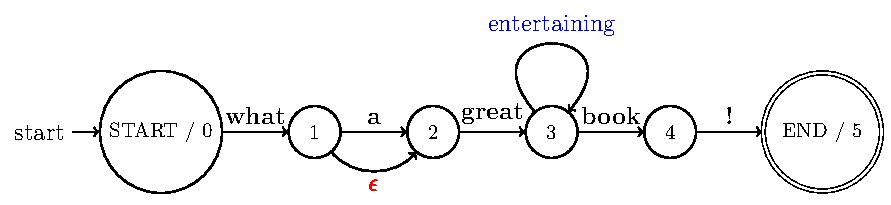
\includegraphics[width=14cm]{pdfs/generated/generic_nfa_linear_chain/main.pdf}
  \caption{Linear-chain NFA with
    self-loop (blue), $\epsilon$ (red) and main-path (black) transitions; figure
    adapted from \citet{schwartz2018sopa}}
  \label{fig:fa}
\end{figure}

\subsection{Linear-chain WFAs}

\label{section:sopa_lc_wfa}

In regards to the \ac{wfas} used in \ac{sopa}, \citet{schwartz2018sopa} utilize
linear-chain \ac{wfas} where each linear-chain \ac{wfa} is allotted a sequence of
$|\mathcal{Q}|$ states. Each state $i$ in the linear-chain \ac{wfa} has three
possible outgoing transitions; namely a \textbf{self-loop transition} which
consumes a token but stays in the same state $i$, an
\textbf{$\bm{\epsilon}$-transition} which does not consume a token but transitions to
state $i+1$ and a \textbf{main-path transition} which consumes a specific token
and transitions to state $i+1$. Furthermore, \citet{schwartz2018sopa} utilize
only the max-sum and max-product semirings in their linear-chain \ac{wfas}. Figure
\ref{fig:fa} shows a sample \ac{nfa} extracted from the aforementioned linear-chain
\ac{wfa} with all three aforementioned transitions, which could accept
strings such as \texttt{"what a great book !"} and \texttt{"what a great
  entertaining book !"}.

To more concretely express these transitions, \citet{schwartz2018sopa} provide
the following formulation of the transition matrix $\bm{\Gamma}$ under the
linear-chain structure. Here, $\bm{\Gamma}(x)$ represents a $|Q|\times|Q|$ matrix
containing transition scores when consuming an input token $x$. $[\bm{\Gamma}(x)]_{i,j}$
corresponds to the cell value in $\bm{\Gamma}(x)$ for row $i$ and column
$j$ and represents the transition score when consuming token $x$ and
transitioning from state $i$ to $j$.

\begin{equation}
  \label{eq:sopa_transition_matrix_main}
  [\bm{\Gamma}(x)]_{i,j} =
  \begin{cases}
    \bm{u}_i \cdot \bm{v}_x + a_i  & \text{if } j = i \text{ (self-loop transition),} \\
    \bm{w}_i \cdot \bm{v}_x + b_i  & \text{if } j = i + 1 \text{ (main-path transition),} \\
    \bar{0} & \text{otherwise.}
  \end{cases}
\end{equation}

Here, $\bm{u}_i$ and $\bm{w}_i$ are learnable vectors and $a_i$ and $b_i$ are
learnable scalar biases parameterizing transitions out of state $i$. $\bm{v}_x$
represents the word embedding for token $x$ and $\bar{0}$ represents the zero
value in the semiring used as per Definition \ref{def:semiring}. Similarly,
$\epsilon$-transitions are parameterized with the following representation in
$\bm{\Gamma}$:

\begin{equation}
  \label{eq:sopa_transition_matrix_epsilon}
  [\bm{\Gamma}(\epsilon)]_{i,j} =
  \begin{cases}
    c_i  & \text{if } j = i + 1 \text{ ($\epsilon$-transition)} \\
    \bar{0} & \text{otherwise.}
  \end{cases}
\end{equation}

Here, $c_i$ represents a learnable scalar bias for $\epsilon$-transitions out of
state $i$. Next, \citet{schwartz2018sopa} fix the initial vector $\bm{\lambda} =
[\bar{1}, \bar{0}, \ldots, \bar{0}]$ and the final vector $\bm{\rho} = [\bar{0},
\bar{0}, \ldots, \bar{1}]$, where $\bar{1}$ and $\bar{0}$ represent the one and
zero values specified in the semiring as per Definition \ref{def:semiring}.
Ultimately, these are formalisms to imply that there only exists one start and
one accepting state and these are present at both extremes of the linear-chain
\ac{wfa}; which is ultimately consistent with the linear-chain definition as per Definition
\ref{def:lfa}.

The aforementioned constraints in the linear-chain \ac{wfa} structure result in the
transition matrix $\bm{\Gamma}$ being reduced to a sparse diagonal matrix.
Correspondingly, the runtime of the Viterbi algorithm under the linear-chain
\ac{wfas} gets reduced to $O(|Q||\bm{x}|)$ compared to the original runtime in
Remark \ref{rmk:old_runtime}. Finally, it is worth noting that \citet[Page 3,
Section 3.1]{schwartz2018sopa} refer to the linear-chain \ac{wfas} simply as
\textit{``patterns''}. For brevity and consistency, we refer to linear-chain
\ac{wfas} as patterns interchangeably.

\subsection{Document score}

\label{section:sopa_doc_score}

Since \ac{sopa} was intended to compute scores for entire documents and not just
short strings, \citet[Page 3, Section 3.2]{schwartz2018sopa} propose computing
the string score, as per Definition \ref{def:string_score}, over all consecutive
substrings in the document which ultimately returns a document score
$s_{\text{doc}}(\bm{y})$ for an arbitrary document $\bm{y}$. The document score
$s_{\text{doc}}(\bm{y})$ for a linear-chain \ac{wfa} would represent an
aggregated score over all consecutive substrings and would therefore also depend
on the semiring used in the \ac{wfas}. In the case of max-based semirings using
the Viterbi algorithm, the document score $s_{\text{doc}}(\bm{y})$ would reflect
the highest path score corresponding to a substring in document $\bm{y}$.

\subsection{Computational graph}

\label{section:sopa_cg}

To explain the overall computational graph of the \ac{sopa} model, we refer to the
visualization shown in Figure \ref{fig:sopa} with two \ac{wfas} highlighted in
blue and red. The \ac{wfas} compute the aforementioned document scores as they
traverse the document. Given max-based semirings, the max-pooled scores
accumulate in an output layer as shown on the top of Figure \ref{fig:sopa}.
After traversing the full document, the max-pooled scores are passed through a
\ac{mlp} which conducts the final classification to an output label. It is worth
noting that without $\epsilon$-transitions and self-loops, a linear-chain
\ac{wfa} with $|\mathcal{Q}|$ states should always consume $\mathcal{|Q|}-1$
tokens. However, by allowing the aforementioned special transitions; it is
possible for strings of variable lengths to be consumed since an
$\epsilon$-transition can transition to the next state without consuming a token
while a self-loop can consume a token without transitioning to the next state.
This is indeed the case for Pattern 2 in Figure \ref{fig:sopa}, when a self-loop
is encountered in the transition from the token \textit{``and''} to the token
\textit{``most''}.

\begin{figure}[t]
  \centering
  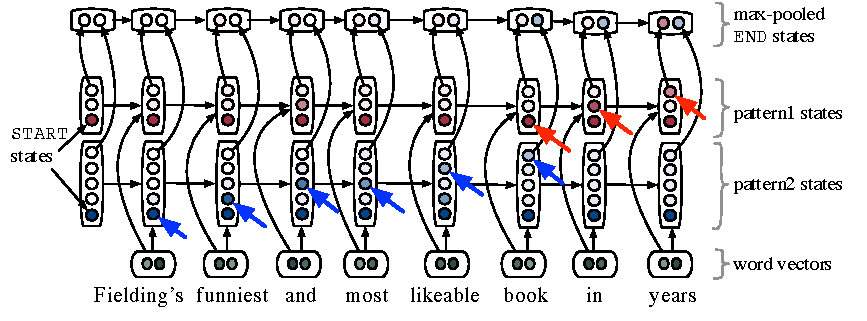
\includegraphics[width=14cm]{pdfs/borrowed/sopa_computational_graph.pdf}
  \caption{SoPa's partial computational graph with two constituent
    WFAs highlighted in blue and red; figure taken from
    \citet{schwartz2018sopa}}
  \label{fig:sopa}
\end{figure}

\subsection{Patterns hyperparameter $P$}

Training the \ac{sopa} model requires both commonly used and special hyperparameters.
Commonly used hyperparameters include the learning rate, neuron dropout and word
dropout probabilities. A special hyperparameter unique to the \ac{sopa} model is the
patterns hyperparameter $P$ which contains information on the number of
linear-chain \ac{wfas} and the number of states allotted to each of them. The
hyperparameter $P$ is encoded with the following syntax:
\texttt{Length$_{1}$-Count$_{1}$\_$\dots$\_Length$_{k}$-Count$_{k}$}. An example
of this hyperparameter $P$ is \texttt{5-15\_4-10\_3-5}, which would signify 15
patterns with 5 states each, 10 patterns with 4 states each and 5 patterns with
3 states each.

\subsection{Transparency}

\label{section:sopa_transparency}

Since we expounded on \ac{xai} in Section \ref{section:xai} and made a case for
viewing \ac{ml} models from the lens of \ac{xai}, it would only make sense to extend the
same standards to the \ac{sopa} model. Based on the arguments made by
\citet{arrieta2020explainable}, we can classify the \ac{sopa} model as a black-box
model since it closely resembles \ac{rnn}s and \ac{cnn}s; and a strong case has already
been made in \citet{arrieta2020explainable} regarding the black-box natures of both \ac{rnn}s and \ac{cnn}s.
Naturally, this would imply that post-hoc explainability techniques are required to
explain the \ac{sopa} model.

\subsection{Explainability}

\label{section:sopa_post_hoc}

In their study, \citet[Page 7, Section 7]{schwartz2018sopa} describe two simple
post-hoc explainability techniques for the \ac{sopa} model. One method involves the
usage of back-pointers during the Viterbi computation to determine the patterns
and substrings in a document which contributed the highest pattern scores.
Another method involves zeroing out the corresponding patterns scores via the
occlusion sensitivity method to determine which pattern had the greatest impact
on each classification decision.

Using the post-hoc explainability taxonomies described in Section
\ref{section:xai_techniques}, we can correspondingly classify the explainability
techniques presented in \citet{schwartz2018sopa} using terminology consistent
with \ac{xai} research. The first explainability technique uses individual text
samples to determine the highest scoring substrings in documents; as well as the
patterns or \ac{wfas} corresponding to them. Since this analysis is conducted at
an individual document level and is never synthesized to a more global context,
we would classify this under the local explanations explainability technique.
The next technique involves an occlusion or sensitivity analysis over all
patterns and documents to determine which pattern had the greatest impact for
each class. Since this involves systematic perturbation to determine the
importance of pattern features, we would classify this technique as a feature
relevance explainability technique. While the target audience of these
explainability techniques is not explicitly mentioned in their study, we infer
that the target audience for these techniques is likely to be average end-users
since the outputs of these post-hoc explainability techniques are generally easy
to understand.

In order to objectively probe the quality of the post-hoc explainability
techniques proposed by \citet{schwartz2018sopa}, we utilize the three guidelines
provided in Section \ref{section:xai_metrics}; namely that a good explanation
should be constrictive, causal and selective. For the constrictive quality, it
is likely that the explainability techniques do not meet this criterion since
they only highlight individual features that were important for \ac{sopa}, and
do not necessarily go into detail regarding why these features superseded
adjacent features. Next, the explainability techniques likely fulfill the
criterion of providing causal links; since they can identify substrings causing
the maximum perturbations in the \ac{mlp} of \ac{sopa}. Finally, the explainability
techniques likely fulfill the criterion of being selective since they only
provide the most important features for an explanation.

Overall, we gather three key limitations regarding the explainability techniques
of \ac{sopa}. Firstly, we find them to be localized because the local
explanations component of explainability was not synthesized to a global
context. Next, we find them to be indirect because of their reliance on the
feature relevance explainability technique which is known to be indirect as per
Remark \ref{rmk:feature_relevance_indirect}. Finally, as per our evaluation of
explainability using the three aforementioned guidelines; we find the
explainability techniques likely do not meet the constrictive criterion in the
guidelines for good explanations.

% LocalWords:  automata understandability simulatable decomposable regressors
% LocalWords:  algorithmically Simulatability Decomposability interpretability
% LocalWords:  Explainability XAI explainability subspaces Interpretable STE's
% LocalWords:  Shapley tradeoff performant Quantized piecewise quantized NFA
% LocalWords:  Contrastingly semiring tokenization Semirings semirings Kleene
% LocalWords:  substring Viterbi WFAs parameterizing formalisms substrings
% LocalWords:  hyperparameter hyperparameters

%%% Local Variables: 
%%% mode: latex
%%% TeX-master: "main"
%%% End: 
\chapter{Methodologies}

\label{chapter:methodologies}

In this chapter, we describe the methodologies used in this thesis.
Comprehensive source code reflecting these methodologies can be found in our
public GitHub
repository\footnote{https://github.com/atreyasha/spp-explainability}.

\section{Facebook Multilingual Task Oriented Dialog}

\citet{schuster-etal-2019-cross-lingual} originally released the Facebook
Multilingual Task Oriented Dialog (FMTOD) data set to encourage research in
cross-lingual transfer learning for Natural Language Understanding (NLU) tasks;
specifically from from high-resource to low-resource languages. The authors
released the FMTOD data set with English as the high-resource language providing
$\sim$43k annotated utterances, and Spanish and Thai as low-resource languages
providing a total of $\sim$14k utterances. Furthermore, they streamlined the
data set on two key tasks; namely intent detection and textual slot filling. In
this thesis, we focus solely on the English language intent detection task in
the FMTOD data set. This intent detection task entails a multi-label sequence
classification task with a total of 12 classes from alarm, reminder and
weather-related domains.

\subsection{Motivation}

We chose to work with the FMTOD data set since it is both a recently released
and well-studied data set
\citep{schuster-etal-2019-cross-lingual,zhang2019joint,zhang-etal-2020-intent}.
We focus on the English language intent classification task since it is a
relatively straightforward task which allows us to place a greater focus on
performance and explainability. Furthermore, the English language subset entails
the highest resources in the FMTOD data set. Finally, we find the FMTOD data
set's intent detection classification especially attractive because it allows us
to test the SoPa++ model on a multi-class NLU problem; which is significantly
different from the focus on binary classification sentiment detection tasks in
SoPa \citep{schwartz2018sopa}.

\subsection{Preprocessing}

We enumerate our preprocessing steps below:

\begin{enumerate}{}
  \item Similar to \citet{schwartz2018sopa}, we convert all FMTOD text samples
  to a lowercased format. This assists in simplifying the data set further.
  \item Next, we search through the pre-provided training, validation and test
  data partitions to remove duplicates within each partition.
  \item Finally, we remove data duplicates which overlap between partitions.
  During this step, we do not remove any cross-partition duplicates from the
  test partition in order to keep it as similar as possible to the original test
  partition. This comes into importance later when we compare performance
  evaluations on the test set with other studies.
\end{enumerate}

\begin{figure}[t]
  \centering
  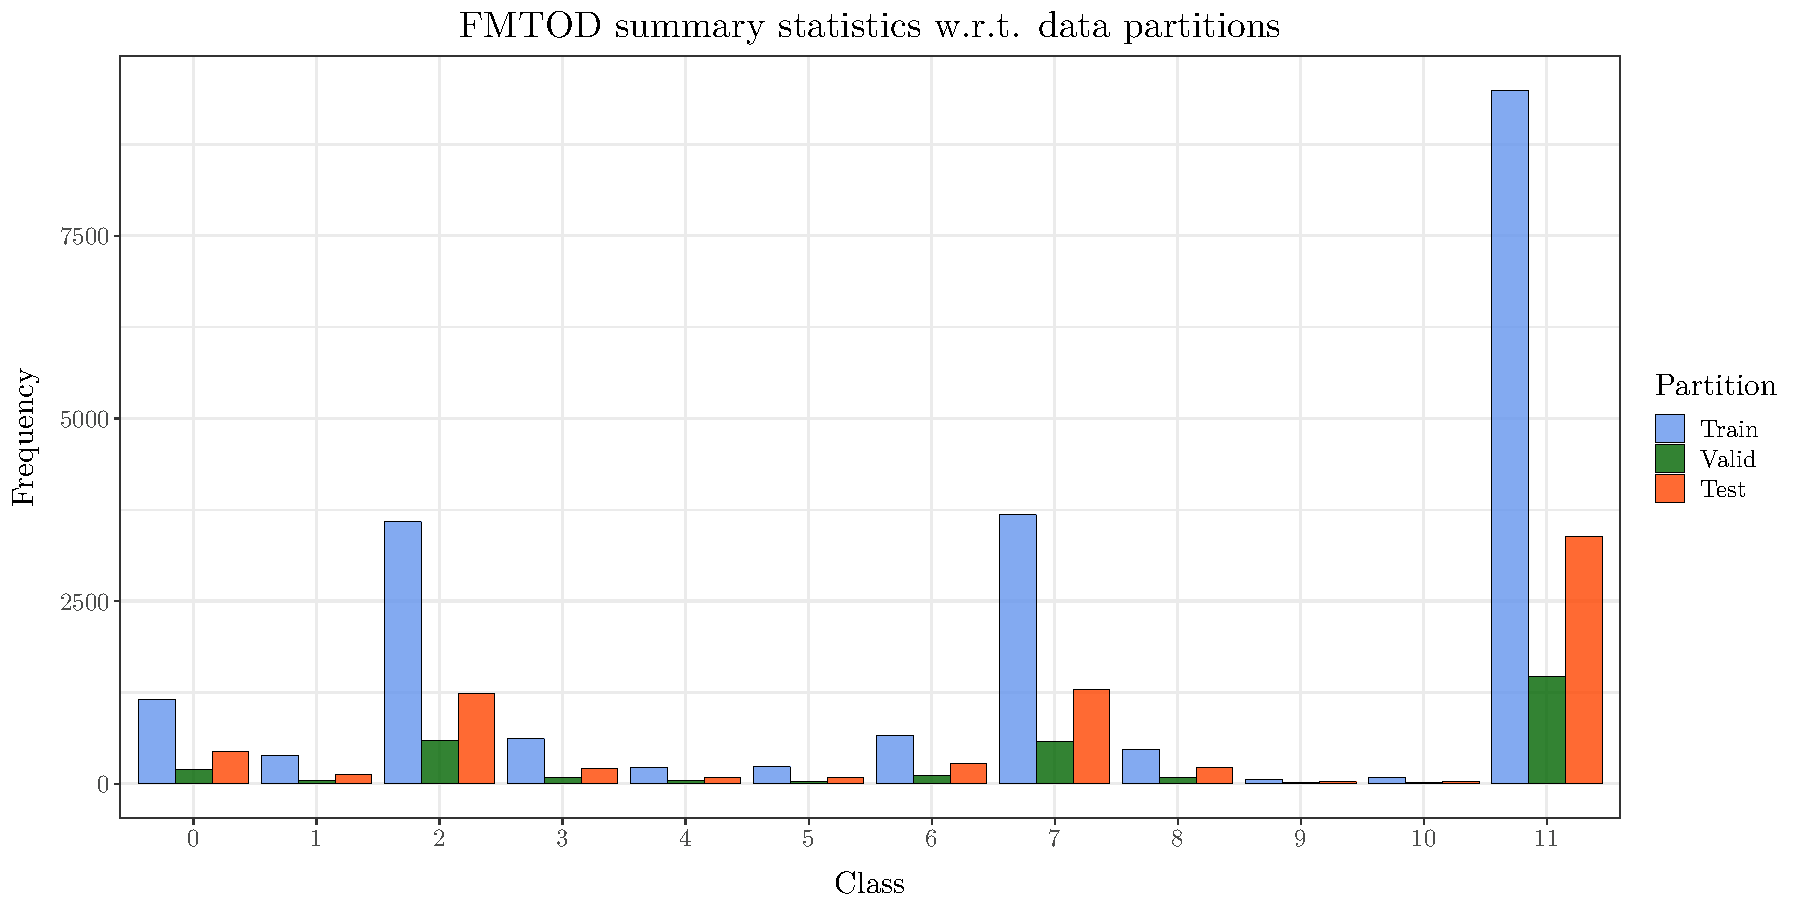
\includegraphics[width=14cm]{pdfs/generated/fmtod_summary_statistics.pdf}
  \caption{Data distribution of the preprocessed FMTOD data set grouped by
    classes and partitions}
  \label{fig:fmtod}
\end{figure}

\begin{table}[t!]
  \centering
  \begin{tabular}{lllll}
    \toprule
    Class and description & Train & Validation & Test & $\Sigma$ \\
    \midrule
    0: \texttt{alarm/cancel\_alarm} & 1157 & 190 & 444 & 1791 \\
    1: \texttt{alarm/modify\_alarm} & 393 & 51 & 122 & 566 \\
    2: \texttt{alarm/set\_alarm} & 3584 & 596 & 1236 & 5416 \\
    3: \texttt{alarm/show\_alarms} & 619 & 83 & 212 & 914 \\
    4: \texttt{alarm/snooze\_alarm} & 228 & 49 & 89 & 366 \\
    5: \texttt{alarm/time\_left\_on\_alarm} & 233 & 30 & 81 & 344 \\
    6: \texttt{reminder/cancel\_reminder} & 662 & 114 & 284 & 1060 \\
    7: \texttt{reminder/set\_reminder} & 3681 & 581 & 1287 & 5549 \\
    8: \texttt{reminder/show\_reminders} & 474 & 82 & 217 & 773 \\
    9: \texttt{weather/check\_sunrise} & 63 & 13 & 25 & 101 \\
    10: \texttt{weather/check\_sunset} & 88 & 11 & 37 & 136 \\
    11: \texttt{weather/find} & 9490 & 1462 & 3386 & 14338 \\[5pt]
    \hline \hline \\[-10pt]
    $\Sigma$ & 20672 & 3262 & 7420 & 31354 \\
    \bottomrule
  \end{tabular}
  \caption{Frequency of the preprocessed FMTOD data set classes grouped by
    partitions; $\Sigma$ signifies the cumulative frequency statistic}
  \label{tab:fmtod}
\end{table}

Many of the duplicates observed were already present in the original FMTOD data
set, with additional duplicates being created from the initial lowercasing step.
After preprocessing, we obtain a lowercased variant of the FMTOD data set with
strictly unique data partitions. In the next section, we describe the summary
statistics of the preprocessed FMTOD data set.

\begin{table}[t!]
  \centering
  \begin{threeparttable}
    \begin{tabular}{lll}
      \toprule
      Class and description & Utterance length$^{\dagger}$ & Example$^{\ddagger}$ \\
      \midrule
      0: \texttt{alarm/cancel\_alarm} & 5.6 $\pm$ 1.9 & cancel weekly alarm \\
      1: \texttt{alarm/modify\_alarm} & 7.1 $\pm$ 2.5 & change alarm time \\
      2: \texttt{alarm/set\_alarm} & 7.5 $\pm$ 2.5 & please set the new alarm \\
      3: \texttt{alarm/show\_alarms} & 6.9 $\pm$ 2.2 & check my alarms. \\
      4: \texttt{alarm/snooze\_alarm} & 6.1 $\pm$ 2.1 & pause alarm please \\
      5: \texttt{alarm/time\_left\_on\_alarm} & 8.6 $\pm$ 2.1  & minutes left on my alarm \\
      6: \texttt{reminder/cancel\_reminder} & 6.6 $\pm$ 2.2 & clear all reminders. \\
      7: \texttt{reminder/set\_reminder} & 8.9 $\pm$ 2.5 & birthday reminders \\
      8: \texttt{reminder/show\_reminders} & 6.8 $\pm$ 2.2 & list all reminders \\
      9: \texttt{weather/check\_sunrise} & 6.7 $\pm$ 1.7 & when is sunrise \\
      10: \texttt{weather/check\_sunset} & 6.7 $\pm$ 1.7 & when is dusk \\
      11: \texttt{weather/find} & 7.8 $\pm$ 2.3 & jacket needed? \\[5pt]
      \hline \hline \\[-10pt]
      $\mu$ & 7.7 $\pm$ 2.5 & \textemdash \\
      \bottomrule
    \end{tabular}
    \begin{tablenotes}[flushleft]
      \footnotesize
      \item $^{\dagger}$Summary statistics follow the mean $\pm$
      standard-deviation format
      \item $^{\ddagger}$Short and simple examples were chosen for brevity and
      formatting purposes
    \end{tablenotes}
  \end{threeparttable}
  \caption{Tabular summary of utterance length statistics and examples for FMTOD
    data classes; $\mu$ signifies the cumulative summary statistics}
  \label{tab:fmtod-examples}
\end{table}

\begin{table}[t!]
  \centering \def\arraystretch{1.3}
  \begin{tabular}{L{0.27\linewidth} L{0.45\linewidth} l}
    \toprule
    Study & Summary & Accuracy \\
    \midrule
    \citet{schuster-etal-2019-cross-lingual} & BiLSTM jointly trained on both the slot filling and intent detection English language tasks & 99.1$\%$ \\
    \citet{zhang2019joint} & BERT along with various decoders jointly fine-tuned on both the slot filling and intent detection English language tasks & 96.6--98.9$\%$ \\
    \citet{zhang-etal-2020-intent} & RoBERTa and XLM-RoBERTa fine-tuned on the English language and multilingual intent detection tasks respectively along with WikiHow pre-training & 99.3--99.5$\%$ \\
    \bottomrule
  \end{tabular}
  \caption{Tabular summary of studies that addressed the FMTOD intent detection
    English language task, along with their relevant summaries and accuracy
    range(s)}
  \label{tab:fmtod-results}
\end{table}

\subsection{Summary statistics}

Figure \ref{fig:fmtod} shows the summary statistics of the preprocessed FMTOD
data set grouped by classes and data set partitions. Similarly, Table
\ref{tab:fmtod} shows the same summary statistics in a tabular form with
explicit frequencies. Based on the summary statistics, we can observe that the
preprocessed FMTOD data set is significantly imbalanced with $\sim$45$\%$ of
samples falling into Class 11 alone. We take this observation into consideration
in later sections and apply fixes to mitigate this data imbalance. In addition,
we observe from Table \ref{tab:fmtod-examples} that input utterances in the
preprocessed FMTOD data set are generally short; with a mean input utterance
length of 7.7 and a standard deviation of 2.5 tokens. Utterance length summary
statistics were computed with the assistance of NLTK's default \texttt{Treebank}
word tokenizer \citep{bird-loper-2004-nltk}.

\subsection{Performance range}

Several studies have optimized deep learning models on the FMTOD English
language intent classification task using a variety of models from BiLSTMs to
XLM-RoBERTa
\citep{schuster-etal-2019-cross-lingual,zhang2019joint,zhang-etal-2020-intent}.
Table \ref{tab:fmtod-results} summarizes these studies along with their reported
accuracy scores on the FMTOD English language intent classification task. Based
on the presented results from these recent studies, we can infer that the
general competitive accuracy range for the FMTOD English language intent
classification task is from 96.6$\%$ to 99.5$\%$.

\section{SoPa++}

In this section we describe our SoPa++ model's architecture and present both
similarities and differences compared to the SoPa model in
\citet{schwartz2018sopa}.

\subsection{Tokenization and word embeddings}

Similar to \citet{schwartz2018sopa}, we utilize NLTK's default \texttt{Treebank} word
tokenizer \citep{bird-loper-2004-nltk} to conduct tokenization of input
utterances into word-level tokens. While \citet{schwartz2018sopa} utilize GloVe
840B 300-dimensional true-cased embeddings, we utilize GloVe 6B 300-dimensional
uncased word-level embeddings \citep{pennington2014glove} to project the input
tokens in utterances to continuous numerical spaces. We utilized this smaller
subset of word-level embeddings since it allowed us to work with lower-cased
words, as well as experiment with a variety of embedding dimensions during our
development phase.

\subsection{$\omega$-Weighted finite state automaton}

As mentioned in Section \ref{section:soft-patterns}, \citet{schwartz2018sopa}
constructed the SoPa model with an ensemble of linear-chain WFAs which permitted
both epsilon and self-loop transitions. As noted in Section
\ref{section:sopa-model-specs}, epsilon and self-loop transitions are useful
constructs in abstracting WFAs and allowing them to match variable length
strings. However based on our experimentation during our development phase, we
observed a key concern that the highest scoring paths in the WFAs in SoPa tended
to have a large variation of string lengths due to the effect of both
epsilon-transitions and self-loops. We believe that this reduced the impact
of SoPa's explainability methods and as a result, the first change we
decided for was to remove both epsilon and self-loop transitions. With this
change, we could at least ensure that each WFA would match strings of a fixed length.

However, matching strings of fixed lengths could also be seen as a form of overfitting in
the model; since a model could simply memorize short strings or phrases and
would not necessarily "learn" to generalize. To address this concern, we
decicded to include a new type of transition within the now strict linear-chain
WFAs; namely the wildcard transition which we define here as a
$\omega$-transition. Allowing for such a transition was only natural since
wildcards are already crucial parts of regular expressions; which as we
mentioned are equivalent to FAs. With this, we provide the following amended
definition for a $\omega$-WFA: 

\begin{definition}[$\omega$-Weighted finite-state automaton]
  \label{def:w-wsa}
  A $\omega$-weighted finite-state automaton over a semiring $\mathbb{K}$ is a 5-tuple
  $\mathcal{A} = \langle \Sigma, \mathcal{Q}, \Gamma, \lambda, \rho \rangle$,
  with:

  \begin{itemize}
    \itemsep0em
    \item[--] a finite input alphabet $\Sigma$;
    \item[--] a finite state set $\mathcal{Q}$;
    \item[--] transition weights $\Gamma: \mathcal{Q} \times \mathcal{Q} \times
    (\Sigma \cup \{\omega\}) \rightarrow \mathbb{K}$;
    \item[--] initial weights $\lambda: \mathcal{Q} \rightarrow \mathbb{K}$;
    \item[--] and final weights $\rho: \mathcal{Q} \rightarrow \mathbb{K}$.
  \end{itemize}

  \begin{remark}
    An $\omega$ transition is equivalent to a wildcard transition, which
    consumes an arbitrary token input and moves to the next state
  \end{remark}

  \begin{remark}
    Besides the inclusion of the $\omega$-transition and removal of the
    $\epsilon$-transition, an $\omega$-WFA has all of the same characteristics
    as the WFA defined in Definition \ref{def:wfa}.
  \end{remark}  
\end{definition}

With the removal of the epsilon and self-loop transitions, we were able to allow
for fixed string length matches to our WFAs. In addition, with the introduction
of the $\omega$-WFA, we are able to add a layer of generalization such that any
token input could possibly be accepted. Finally, similar to
\citet{schwartz2018sopa} we enforce that our $\omega$-WFAs all have a strict
linear-chain structure. They are now considered strict since we removed the
option of self-loop transitions.

%%% Local Variables: 
%%% mode: latex
%%% TeX-master: "main"
%%% End: 
\chapter{Results}

\label{chapter:results}

In this chapter, we focus on summarizing the results of our aforementioned
methodologies. As a note, we do not dive deep into answering our research
questions here. Instead, we simply use this chapter to report on our results and
we answer our research questions in the next chapter.

\section{RQ1: Evaluating performance of SoPa++}

Following our methodologies, we conducted a grid-search training paradigm where
we varied our patterns and $\tau$-threshold parameters to obtain a total of 15
different modelling runs. Given that we repeated unique model run 10 times, we
ultimately ran our grid-search for 150 model runs. This process took roughly 24
hours on a single NVIDIA GeForce GTX 1080 Ti GPU running light, medium and heavy
model runs concurrently.

\subsection{Training}

We first describe the results of our training. Figure \ref{fig:results_training}
shows the progress of the validation accuracy against training updates. The
different coloured lines indicate the various initial random seeds assigned to
the particulat model run. We can observe that increasing the $\tau$ value from 0
to 1 tends to decrease the overall validation accuracy profile. Correspondingly,
we can also observe that the larger model tends to have a higher validation
accuracy profile compared to the smaller models. We refer to the pattern
hyperparameter as $P$ in Figure \ref{fig:results_training}. Finally, we can
observe that the larger models tend to have an earlier convergence or
early-stopping window compared to the smaller models.

\subsection{Evaluation}

In regards to the evaluation of SoPa++ performance, we can refer to Table
\ref{tab:results_evaluation} for a tabular summary of test accuracies across the
light, medium and heavy model variants grouped by the various $\tau$-thresholds.
The exact specification of the light, medium and heavy model variants were
described in Section \ref{section:spp_training}. Here, we can observe that the
best performing models were the heavy models with $\tau$=0.0 and $\tau$=0.25
and the medium model with $\tau$=0.0. We can observe that test accuracies
generally show a decreasing trend as we increase the $\tau$-threshold.
Correspondingly, we can observe a decreasing performance trend as we decrease
the size of the model from heavy to light models. We can also observe that the
standard deviations in performance are generally similar.

\begin{figure}[t!]
  \centering
  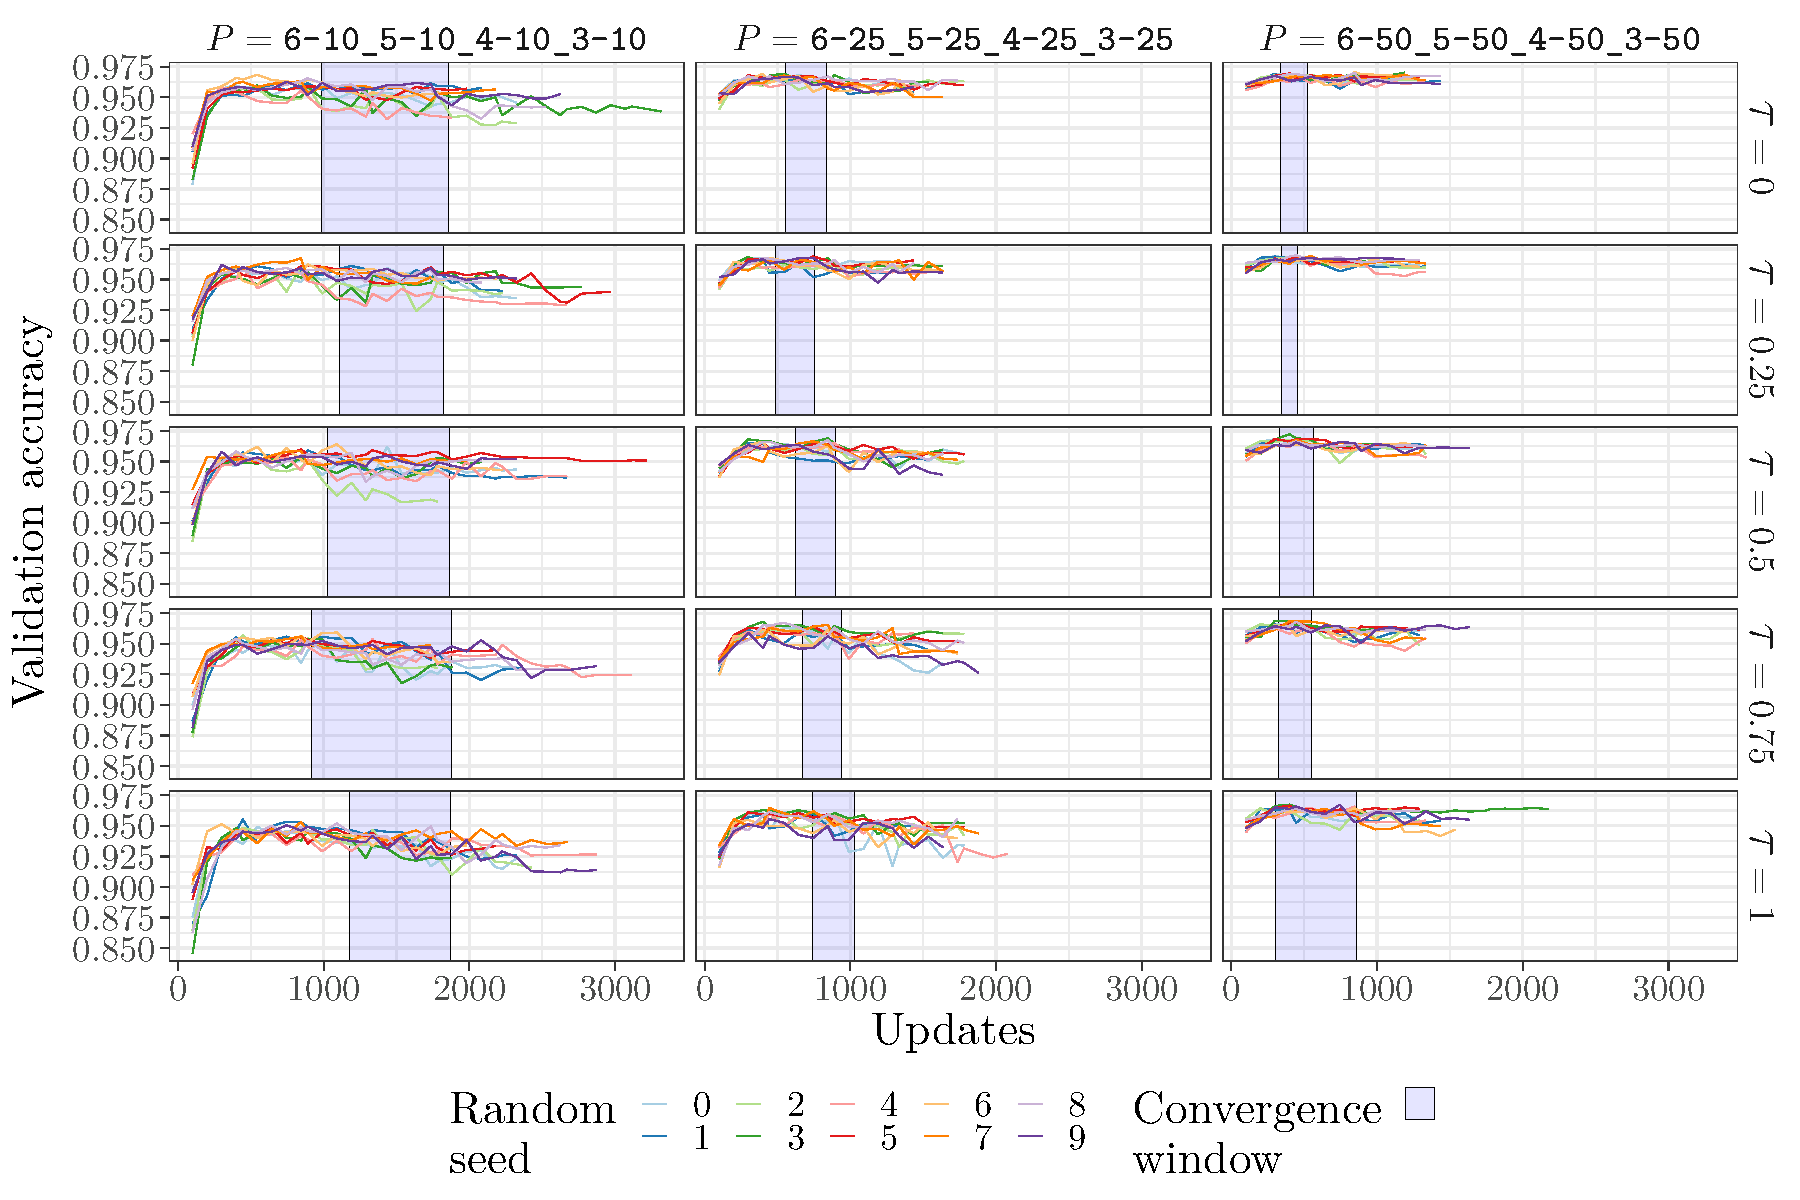
\includegraphics[width=14cm]{pdfs/generated/train_spp_grid_1617362157.pdf}
  \caption{Visualization of validation accuracy against number of training
    updates for grid-search grouped by pattern hyperparameters and $\tau$-thresholds}
  \label{fig:results_training}
\end{figure}

\begin{table}[t!]
  \centering \def\arraystretch{1.3}
  \small
  \begin{tabular}{lllllll}
    \toprule
    && \multicolumn{5}{c}{Accuracy in $\%$ with mean $\pm$ standard-deviation} \\
    \cline{3-7} \\[-10pt]
    Model & Parameters & $\tau$=0.0 & $\tau$=0.25 & $\tau$=0.5 & $\tau$=0.75 & $\tau$=1.0 \\
    \midrule
    Light & 1,260,292 & 97.6 $\pm$ 0.2 & 97.6 $\pm$ 0.2 & 97.3 $\pm$ 0.2 & 97.0 $\pm$ 0.3 & 96.9 $\pm$ 0.3 \\
    Medium & 1,351,612 & \bm{$98.3 \pm 0.2$} & 98.1 $\pm$ 0.1 & 98.0 $\pm$ 0.2 & 97.9 $\pm$ 0.1 & 97.7 $\pm$ 0.1  \\
    Heavy & 1,503,812 & \bm{$98.3 \pm 0.2$} & \bm{$98.3 \pm 0.2$} & 98.2 $\pm$ 0.2 & 98.1 $\pm$ 0.2 & 98.0 $\pm$ 0.2 \\
    \bottomrule
  \end{tabular}
  \caption{Test accuracies of the SoPa++ models grouped by model sizes and
    $\tau$-thresholds; accuracies and standard deviations were calculated across
  random seed iterations; bold scores show best performing models}
  \label{tab:results_evaluation}
\end{table}

\section{RQ2: Evaluating explanations by simplification}

For evaluating explanations by simplification, we also follow our methodologies.
Firstly, we refer to Figure \ref{fig:explain_evaluate} for a visualization of
all results. We can observe a general trend that SoPa++ and RE proxy accuracies
become more similar to one another as we increase the value of the
$\tau$-threshold. Similarly, we can observe a general trend that the mean
model-pair distances $\overline{\delta_{\sigma}}$ and $\overline{\delta_b}$ both
become smaller as we increase the value of the $\tau$-threshold. In general, we
can observe that the models with more parameters tend to have better test set
accuracies for both SoPa++ and RE proxy models. Similarly, we can observe that
the overall test set performance tends to decrease for SoPa++ but increase for
the RE proxy models as the $\tau$-threshold value is increased. Table
\ref{tab:results_evaluation} shows a tabular summary of test set accuracies and
model-pair distance metrics for both SoPa++ and RE proxy models. 

\begin{figure}[t!]
  \centering
  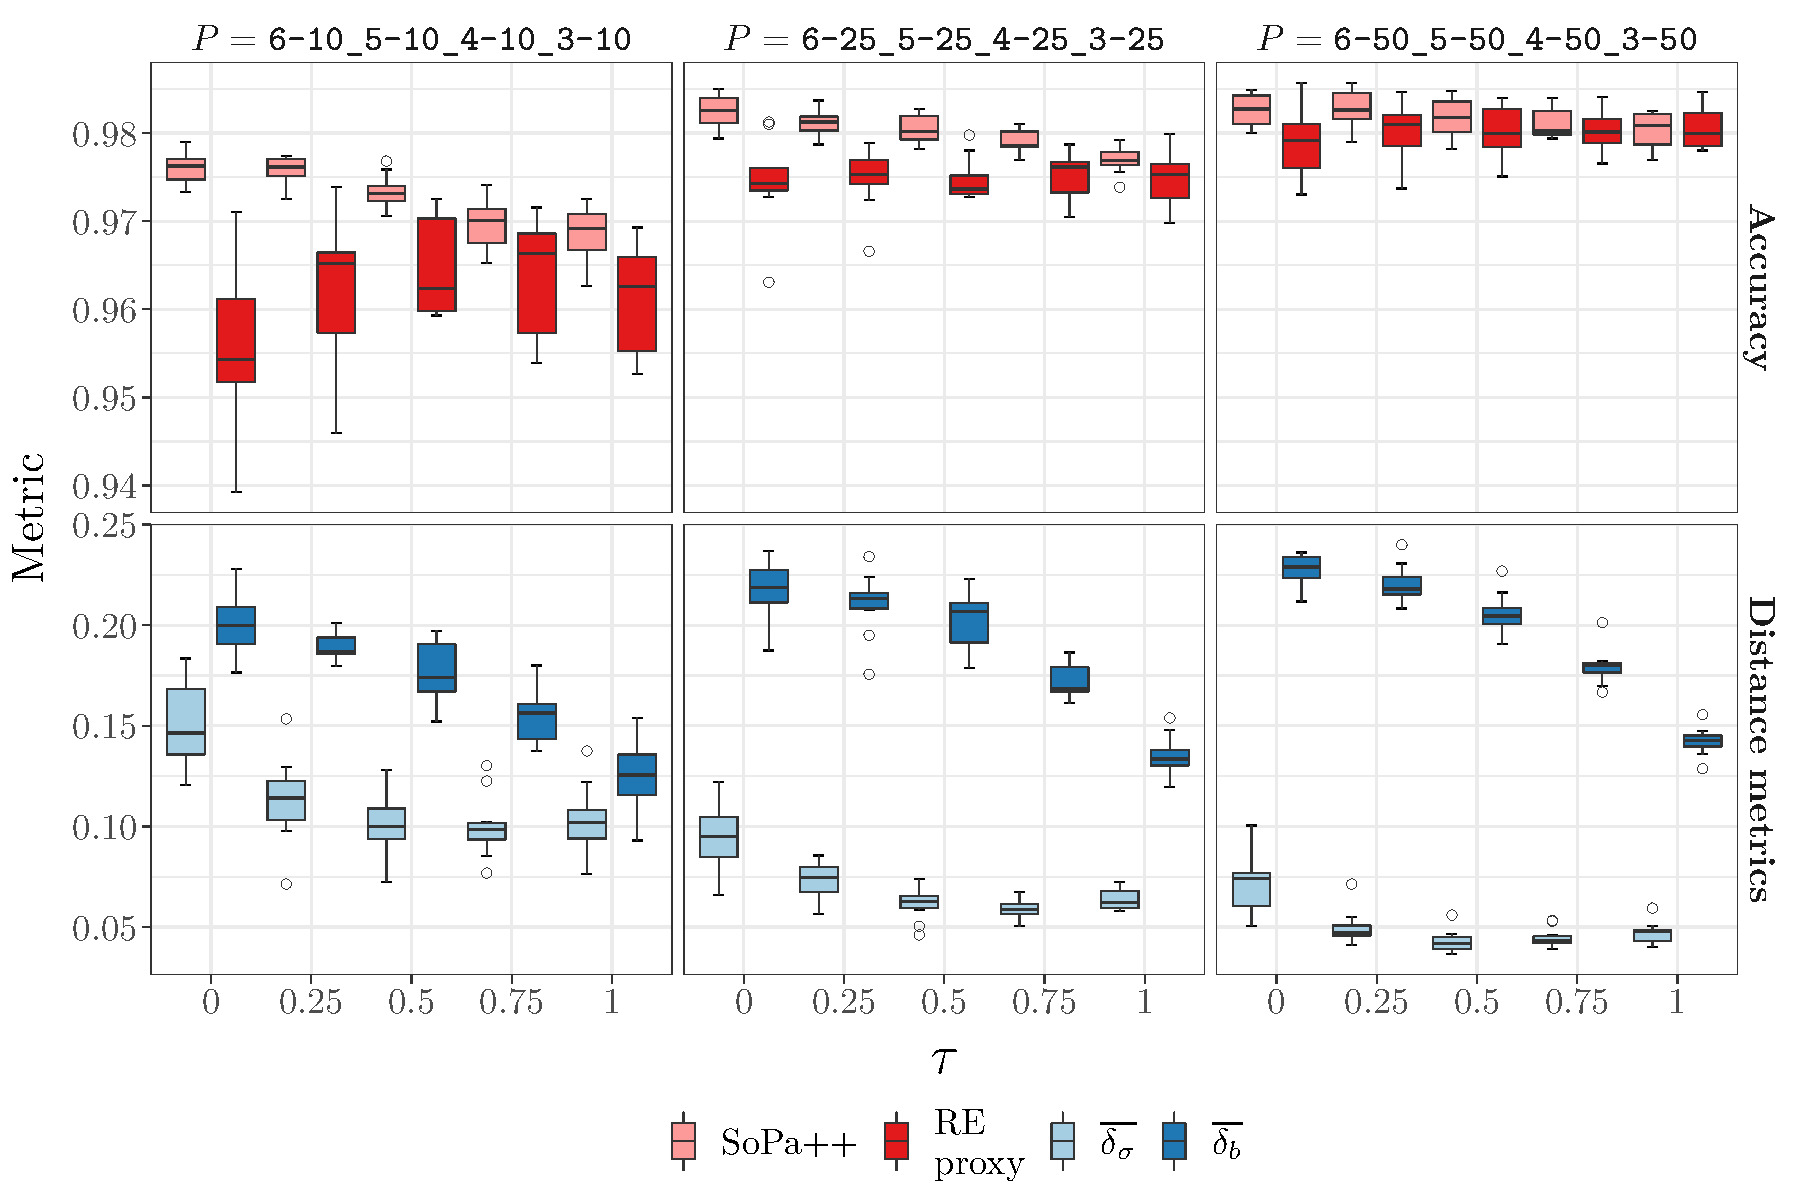
\includegraphics[width=14cm]{pdfs/generated/evaluate_spp_grid_1617375541.pdf}
  \caption{Visualization of accuracy and model-pair distance metrics against
    pattern hyperparameters and $\tau$-thresholds}
  \label{fig:explain_evaluate}
\end{figure}

\begin{table}[t!]
  \centering \def\arraystretch{1.3}
  \small
  \begin{tabular}{lllllll}
    \toprule
    && \multicolumn{5}{c}{Accuracy in $\%$ with mean $\pm$ standard-deviation} \\
    \cline{3-7} \\[-10pt]
    Model & Variant & $\tau$=0.0 & $\tau$=0.25 & $\tau$=0.5 & $\tau$=0.75 & $\tau$=1.0 \\
    \midrule
    Light & SoPa++ & 97.6 $\pm$ 0.2 & 97.6 $\pm$ 0.2 & 97.3 $\pm$ 0.2 & \bm{$97.0 \pm 0.3$} & 96.9 $\pm$ 0.3 \\
    & RE proxy & 95.5 $\pm$ 1.0 & 96.2 $\pm$ 0.8 & 96.5 $\pm$ 0.6 & \bm{$96.3 \pm 0.7$} & 96.1 $\pm$ 0.6 \\
    Medium & SoPa++ & 98.3 $\pm$ 0.2 & 98.1 $\pm$ 0.1 & 98.0 $\pm$ 0.2 & 97.9 $\pm$ 0.1 & \bm{$97.7 \pm 0.1$}  \\
    & RE proxy & 97.4 $\pm$ 0.5 & 97.5 $\pm$ 0.3 & 97.5 $\pm$ 0.2 & 97.5 $\pm$ 0.3 & \bm{$97.5 \pm 0.3$} \\
    Heavy & SoPa++ & 98.3 $\pm$ 0.2 & 98.3 $\pm$ 0.2 & 98.2 $\pm$ 0.2 & \bm{$98.1 \pm 0.2$} & \bm{$98.0 \pm 0.2$} \\
    & RE proxy & 97.9 $\pm$ 0.4 & 98.0 $\pm$ 0.3 & 98.0 $\pm$ 0.3 & \bm{$98.0 \pm 0.2$} & \bm{$98.1 \pm 0.2$} \\
    \bottomrule\\[-13pt]
    && \multicolumn{5}{c}{Metric in $\%$ with mean $\pm$ standard-deviation} \\
    \cline{3-7} \\[-10pt]
    Model & Metric & $\tau$=0.0 & $\tau$=0.25 & $\tau$=0.5 & $\tau$=0.75 & $\tau$=1.0 \\
    \midrule
    Light & $\overline{\delta_{\sigma}}$ & 15.0 $\pm$ 2.3 & 11.3 $\pm$ 2.2 & \bm{$10.0 \pm 1.6$} & \bm{$10.0 \pm 1.6$} & 10.3 $\pm$ 1.8 \\
    & $\overline{\delta_b}$ & 20.1 $\pm$ 1.5 & 18.9 $\pm$ 0.7 & \bm{$17.8 \pm 1.5$} & \bm{$15.5 \pm 1.3$} & 12.4 $\pm$ 1.8 \\
    Medium & $\overline{\delta_{\sigma}}$ & 9.5 $\pm$ 1.7 & 7.3 $\pm$ 0.9 & 6.1 $\pm$ 0.8 & \bm{$5.8 \pm 0.5$} & 6.3 $\pm$ 0.5  \\
    & $\overline{\delta_b}$ & 21.7 $\pm$ 1.5 & 21.0 $\pm$ 1.6 & 20.3 $\pm$ 1.5 & \bm{$17.2 \pm 0.9$} & 13.5 $\pm$ 1.0 \\
    Heavy & $\overline{\delta_{\sigma}}$ & 7.1 $\pm$ 1.5 & 5.0 $\pm$ 0.8 & \bm{$4.3 \pm 0.6$} & 4.5 $\pm$ 0.5 & 4.7 $\pm$ 0.5 \\
    & $\overline{\delta_b}$ & 22.7 $\pm$ 0.9 & 22.0 $\pm$ 1.0 & \bm{$20.6 \pm 1.0$} & 18.0 $\pm$ 0.9 & 14.2 $\pm$ 0.7 \\
    \bottomrule
  \end{tabular}
  \caption{Test accuracies and model-pair distances metrics of the SoPa++ and RE
    proxy models grouped by model sizes and $\tau$-thresholds; accuracies and
    standard deviations were calculated across random seed iterations; bold test
    accuracies show model pairs whose accuracies are closest to one another;
    bold distance metrics show models whose $\overline{\delta_{\sigma}}$ metric
    are closest to zero}
  \label{tab:explain_evaluate_performance}
\end{table}


%%% Local Variables: 
%%% mode: latex
%%% TeX-master: "main"
%%% End: 
\chapter{Discussion}

\label{chapter:discussion}

In this chapter, we interpret the results described from the previous chapter
and discuss their implications in order to answer our research questions.
Similar to the previous chapter, we break this chapter into three sections with
each section addressing one research question. Aside from answering the research
questions, we also gather interesting observations and propose hypotheses which could
motivate future research.

\section{RQ1: Evaluating performance of SoPa++}

To answer our first research question on whether SoPa++ can deliver competitive
performance on the FMTOD English language intent classification task, we compare
the mean performance metrics of our SoPa++ models against those from other
recent studies as mentioned in Section \ref{section:fmtod_performance}.
Referring to our accuracy ranges from Table \ref{tab:results_evaluation}, we
observe that the SoPa++ models show an accuracy range from 97.6-98.3$\%$ for the
best performing models given their respective sizes. This falls into the general
accuracy range of 96.6-99.5$\%$ observed in other studies as per Table
\ref{tab:fmtod_examples}; albeit in the lower end of this spectrum. We can
therefore conclude that SoPa++ offers competitive performance on the FMTOD's
English language intent classification task.

While SoPa++'s performance range falling in the lower end of the aforementioned
spectrum can be seen as disadvantageous, it is worth noting that the models
SoPa++ is being compared against are vastly different. For one, the BERT-based
models shown in Table \ref{tab:fmtod_results} had parameter counts ranging from
$\sim$110-340 million parameters \citep{devlin-etal-2019-bert}; which are
$\sim$100-300 times larger than our SoPa++ models. In addition, models from
\citet{zhang-etal-2020-intent} showed an exceptionally high accuracy of 99.5$\%$
mainly because of pre-training on the external WikiHow data set for general
intent classification tasks. Finally, many of the models described in Table
\ref{tab:fmtod_results} were jointly trained on both FMTOD intent classification
and slot filling tasks; which could have contributed to certain joint-task
performance benefits. These significant differences between SoPa++ and the
aforementioned models should be taken into account when comparing SoPa++'s
performance with other studies. 

\section{RQ2: Evaluating explanations by simplification}

To answer our second research question on whether SoPa++ provides effective
explanations by simplification, we summarize the minimum differences in SoPa++
and RE proxy model-pair performance metrics; as well as the minimum distance
metrics observed as per Table \ref{tab:explain_evaluate_performance}. Regarding
performance metrics, we can observe that lowest accuracy score differences
between SoPa++ and RE proxy model-pairs to be 7$\%$ for small-sized models, 2$\%$
for medium-sized models and 1$\%$ for large-sized models. Regarding distance
metrics, we observe the lowest $\overline{\delta_{\sigma}}$ and
$\overline{\delta_{b}}$ to be 10.0$\%$ and 12.4$\%$ for small-sized models, 5.8
$\%$ and 13.5$\%$ for medium-sized models and 4.3$\%$ and 14.2$\%$ for
large-sized models respectively. These minimum performance metric differences
and distance metrics are typically observed with larger $\tau$-thresholds
ranging from 0.50-1.00. Unlike the case for RQ1, we do not have an objective
range of competitive accuracy differences or distance metrics to compare against
with other studies. As a result, our interpretation of the effectiveness of the
explanations by simplification post-hoc explainability technique will be
subjective. That being said, we still believe that accuracy differences as low
as 1$\%$ and softmax distance norms as small as 4.3$\%$ provide significant
evidence towards a high degree of resemblance between SoPa++ and RE proxy
models. In summary, we find that the explanations by simplification post-hoc
explainability technique in SoPa++ is effective, in particular for medium and
large-sized models with $\tau$-thresholds ranging from 0.50-1.00.

In the interest of objectivity, we would like to provide some perspectives in
which the explanations by simplification technique is not effective. For one,
explanations by simplification as a post-hoc explainability technique as per
Definition \ref{def:explain_simplify} explicitly requires the simplified proxy
model to be more transparent than its antecedent counterpart. While we made a
case for the transparency of the RE proxy model in Section
\ref{section:re_transparency}, one could also provide arguments for the RE proxy
model being non-transparent; especially when the RE lookup layer contains too
many regular expressions for a human to comprehend. This could indeed be the
case for medium and large-sized RE proxy models which have RE lookup layers
containing tens of thousands of "activating" regular expressions. In cases such,
it would not be possible for a human to understand all of the regular
expressions; which could ultimately render the RE proxy model as yet another
black-box model. In such cases, the explanations by simplification post-hoc
explainability technique would likely be ineffective.

With these arguments set aside, we now proceed to discuss some interesting
observations in regards to our results for RQ2. Firstly, we can observe the
performance-interpretability tradeoff from Section
\ref{section:performance_interpretability_tradeoff} in Table
\ref{tab:explain_evaluate_performance} with the more transparent RE proxy models
consistently performing worse than their black-box SoPa++ counterparts; with the
exception of the large-sized model-pair with $\tau$=1.00 where the RE proxy
generally outperforms the SoPa++ antecedent model. Next, as per Table
\ref{tab:explain_evaluate_performance}; we observe that RE proxy models tend to
perform better as the $\tau$-threshold increases. We hypothesize that this
occurs mainly because larger $\tau$-threshold forces the memorization of higher
scoring paths which ultimately reduces the chances of the RE proxy model
memorizing superfluous or unimportant regular expressions in the RE lookup
layer. Finally as per Figure \ref{fig:explain_evaluate}, we
observe that the $\overline{\delta_{b}}$ metric continues to decrease as the
$\tau$-threshold increases, while the $\overline{\delta_{\sigma}}$ metric
plateaus beforehand and then slighly increases. This could be seen as
counter-intuitive, since more similar TauSTE binary vectors should imply more
similar softmax distributions. It would be interesting to further explore these
trends with even higher $\tau$-thresholds.

\section{RQ3: Interesting and relevant explanations}

\label{section:discussion_regex}

To answer our third research question on interesting and relevant explanations
derived from SoPa++ on the FMTOD data set, we refer back to our results for this
research question and attempt to interpret them. Since this research question is
more open-ended than the previous two, our approach to answer it will also be
opinionated and subjective. One interesting observation is in the relative
linear weights applied to the TauSTE neurons in Figure \ref{fig:neuron_weights}.
We can observe that weights are generally continously distributed across all
neurons; with some exceptions such as neurons 19, 25 and 17 where the weights
are more skewed towards the alarm, reminder and weather domains respectively.
This implies that SoPa++ and RE proxy models still distribute feature
importances across TauSTE neurons in a highly connective sense; which also implies that
each TauSTE neuron has a non-negligible impact on all classification decisions.

With the identification of the salient TauSTE neurons 19, 25 and 17 specializing
in the alarm, reminder and weather domains respectively; we draw out ten regular
expression samples from RE lookup layer corresponding to each of these neurons
as reflected in Figures \ref{fig:regex_example_neuron_alarm},
\ref{fig:regex_example_neuron_reminder} and
\ref{fig:regex_example_neuron_weather} respectively. To extract interesting and
relevant explanations, we attempt to interpret these sampled regular
expressions. Firstly, we can observe a segmentation of lexical information
between the regular expressions corresponding to these neurons. For example,
many of the regular expressions corresponding to neuron 19 use words related to
alarms such as \textit{"snooze"} and \textit{"clock"}; while those corresponding to neuron 17 use
words related to weather such as \textit{"fahrenheit"} and \textit{"forecast"}. Next, we can
observe transition clustering or branching in sampled regular expressions across
all three TauSTE neurons. This branching phenomenon is interesting because words
in these branches can sometimes have very similar lexical semantics. For
example, in the third regular expression from the bottom in Figure
\ref{fig:regex_example_neuron_weather}, we observe branching with three
different digital tokens \textit{"44"}, \textit{"70"} and \textit{"67"} which
represent the temperatures encountered in the training data. Similarly, the
third regular expression from the top in Figure
\ref{fig:regex_example_neuron_weather} shows branching with the tokens
\textit{"atlanta"}, \textit{"omaha"} and \textit{"hawaii"}, which all represent
locations in the USA encountered in the training data. Finally, we can observe
interesting positional, or possibly syntactic, features in the regular
expressions in Figures \ref{fig:regex_example_neuron_alarm} and
\ref{fig:regex_example_neuron_reminder}; which all have a $\omega$-transition in
the same transition.

Finally, the sampled regular expressions allow us to identify various inductive
biases incorporated by SoPa++ and its RE proxy models from the training data.
Going back to the digital and location-based tokens mentioned in the previous
paragraph, we can observe how the training data induces USA-centric biases
pertaining to locations such as \textit{"atlanta"} and hard-coded Fahrenheit
temperatures such as \textit{"70"}. As a result, we can extrapolate that the
SoPa++ and RE proxy models will likely only perform well on unseen data based in
USA-centric domains since they likely would not have encountered tokens from
non-USA-centric domains. An advantageous aspect of the RE proxy model is that
these inductive biases can be easily identified and also corrected. In the case
of correcting USA-centric locations, we could manually add more non-USA-based
locations in the branching transition of the third regular expression from the
top in Figure \ref{fig:regex_example_neuron_weather}. Another possible inductive
bias could be in the third regular expression from the top in Figure
\ref{fig:regex_example_neuron_alarm}, where the first transition only allows for
the pronoun \textit{"i"}. This inductive bias could be corrected in the RE proxy
model by augmenting it with all other pronouns available in the English
language. Finally, we can propagate these manual corrections in the RE proxy
model back to SoPa++ by copying the word embeddings and transition matrix
diagonals of the biased word to now represent those of the manually added new
words.

%%% Local Variables: 
%%% mode: latex
%%% TeX-master: "main"
%%% End: 
\chapter{Conclusions}

\label{chapter:conclusions}

In this chapter, we summarize and highlight the key findings of this thesis. We
started off this thesis by emphasizing the importance of \ac{xai} research and
correspondingly laid out clear definitions of \ac{xai}-related concepts adapted
from \citet{arrieta2020explainable}. We then drew inspiration from the SoPa
model in \citet{schwartz2018sopa} and focused on improving the SoPa model to
ultimately create our SoPa++ model. The most significant changes in SoPa++
included the modification of linear-chain \ac{wfas} to strict linear-chain
\ac{wfaws}, the replacement of the \ac{mlp} with layer normalization,
\ac{tauste} and linear layers and the introduction of the explanations by
simplification post-hoc explainability technique to create \ac{re} proxy models.
With these changes, we proceeded to answer our three research questions listed
in Section \ref{section:rq}.

Regarding our first research question, we observe that SoPa++'s best accuracy
range on the \ac{fmtod} data set of 97.6-98.3$\%$ falls into the competitive accuracy
range of 96.6-99-5$\%$ based on other recent studies. In this respect, we
conclude that SoPa++ offers competitive performance on the \ac{fmtod} English
language intent classification task.

Regarding our second research question, we compare the accuracy scores and
distance metrics between SoPa++ and \ac{re} proxy model pairs and observe accuracy
differences as low as $\sim$1$\%$ and softmax distance norms as small as $\sim$4$\%$ for
medium and large-sized models with $\tau$-thresholds ranging from 0.50-1.00. We
therefore conclude that the explanations by simplification post-hoc
explainability technique is effective on the \ac{fmtod} English language intent
classification task given larger model sizes and $\tau$-thresholds.

Regarding our third and final research question, we identify salient \ac{tauste}
neurons which received disproportionately large relative linear weights in our
best performing small \ac{re} proxy model. Next, we analyze regular expression
samples in the \ac{re} lookup layer from the aforementioned \ac{re} proxy model
corresponding to these salient neurons. Based on an analysis of these sampled
regular expressions, we observe several interesting phenomena such as lexical
segmentation, branching transitions with tokens having similar lexical semantics
and also the presence of USA-centric inductive biases captured from the training
data.

%%% Local Variables: 
%%% mode: latex
%%% TeX-master: "main"
%%% End: 
\chapter{Further work}

\label{chapter:further_work}

In this final chapter, we address the limitations of our methodologies and
discuss possible future research directions which could be pursued to mitigate
these limitations.

\section{Efficiency}

In this thesis, we showed the effectiveness of simplifying \ac{sopa}++ models into \ac{re}
proxy models. While \ac{sopa}++ models ran very efficiently because of tensor-based
parallelizations and \ac{gpu} hardware-acceleration derived from \texttt{PyTorch}'s
mature computational ecosystem, we observed that the \ac{re} proxy models ran
significantly slower with the main bottleneck being the slow lookup process in
the \ac{re} lookup layer; as was mentioned in Section \ref{section:re_cg}. To
overcome this low efficiency in \ac{re} proxy models, we could recommend three
approaches. One approach could be to save the \ac{re} lookup layer as a data base and
utilize indexed searches to make regular expression searches and lookups much
faster. Another approach could be to attempt multi-threading on the \ac{re}
lookup process; which is likely to be a complex task and would require
experimental tweaking to attain the best efficiencies. The final approach could
be to utilize \ac{gpu}-accelerated regular expression matching algorithms
\citep{wang2011gregex,zu2012gpu,yu2013gpu} to parallelize the overall \ac{re} lookup
layer and its matching functionalities.

\section{Generalization}

Returning back to the last two paragraphs in Section
\ref{section:discussion_regex}, we recall how certain transitions in the \ac{re}
lookup layer tend to be populated with tokens which have similar lexical
semantics. We specifically draw attention to the example of digital temperature
tokens mentioned in the aforementioned paragraphs and how both \ac{sopa}++ and the \ac{re}
proxy model tend to memorize specific digital tokens such as \textit{"44"},
\textit{"70"} and \textit{"67"}. While it is clear that these tokens could be
replaced by any other finite digital tokens, both \ac{sopa}++ and the \ac{re} proxy model
overfit on these particular tokens. It would therefore be of interest to explore
generalizations on these types of tokens. In the case of the aforementioned
digital tokens, we could replace these transitions in the \ac{re} lookup layer with a
generic Perl-compatible regular expression
\texttt{\textbackslash-?[\textbackslash d]+\textbackslash .?[\textbackslash d]*}
which would match digital tokens with arbitrary lengths, period-separated
decimal precision and a possible minus sign. As a result, this transition would
now be able to accomodate various digital tokens with different formats and
scales. It would be interesting to explore similar generalizations on other
branching transitions such as those for commmunicating time. Naturally, this
process would be much more difficult for tokens that do not have consistent
formatting; which could include synonyms and proper nouns.

\section{Modeling}

Currently, the \ac{sopa}++ model conducts classification decisions by max-pooling
document scores from its constitutent strict-linear chain \ac{wfaws}. These
document scores correspondingly reflect substrings in the document but do not
necessarily contain positional information regarding them, such as substring
X occurring after substring Y. While this was not a shortcoming in the generally
short-sequence \ac{fmtod} data set, it could become a hindrance when applying \ac{sopa}++
to longer documents. As a result, it would be interesting to incorporate
positional information alongside the Viterbi algorithm to allow for
classification on longer documents. Another possible extension could be to
extend \ac{sopa}++'s weighted finite-state automata to finite-state transducers;
which are highly similar but return scored seqeuences instead of scored paths.
In this way, \ac{sopa}++ with finite-state transducers could even be used for
sequence-to-sequence tasks; making it viable for other applications in \ac{nlp} such
as Machine Translation.

\section{Explainability}

In regards to explainability, we largely focused on the technical requirements
for showing effective explanations by simplification for the \ac{sopa}++ model. To
evaluate the quality of explanations of \ac{sopa} vs. \ac{sopa}++, we only used the three
guidelines for good explanations as per Section \ref{section:xai_metrics}. While
useful, these are ultimately only guidelines and do not necessarily reflect the
evaluation of explanations perceived by the target audiences of \ac{sopa} and \ac{sopa}++;
which are average end-users and exper-users respectively. As a result, it would
be interesting to conduct a survey on how satisfactory the provided explanations
from \ac{sopa} and \ac{sopa}++ were to these target audiences. This survey could, for
example, be done in a University's department-wide setting using one of the many
well-developed web-based survey tools where participants provide a basic
positive or negative rating on the provided explanations from their assigned
models. Although subjective, this might help to provide a rating of the
explainability techniques of \ac{sopa} and \ac{sopa}++ through their respective target
audiences.

%%% Local Variables: 
%%% mode: latex
%%% TeX-master: "main"
%%% End: 

%----------------------------------------------------------------------------------------
%	BIBLIOGRAPHY
%----------------------------------------------------------------------------------------

\printbibliography[heading=bibintoc]

%----------------------------------------------------------------------------------------

\end{document}  

%%% Local Variables:
%%% mode: latex
%%% TeX-master: t
%%% End: